% ===========================================================================
%  MARK 2.0 Plus -- Software Evolution Report
%
%  Relazione unica del processo di evoluzione applicato a MARK 2.0.
%  Tutto il documento vive in questo file: preambolo, macro, bibliografia
%  (incorporata con filecontents) e contenuto. Restano esterne solo le
%  immagini, sotto figures/ e figures/cfg/.
%
%  Compilare da docs/latex:
%    pdflatex -interaction=nonstopmode mark-2.0-plus-report.tex
%    biber    mark-2.0-plus-report
%    pdflatex -interaction=nonstopmode mark-2.0-plus-report.tex
%    pdflatex -interaction=nonstopmode mark-2.0-plus-report.tex
%
%  Su Overleaf: Compiler = pdfLaTeX, Main document = questo file.
%  I path delle figure sono relativi a docs/latex, che e' anche la directory
%  da cui Overleaf compila.
% ===========================================================================
\documentclass[11pt,a4paper]{article}

% ---------------------------------------------------------------------------
%  Bibliografia incorporata
%
%  Scritta su \jobname.bib alla prima passata di pdflatex e letta poi da biber:
%  cosi' il report resta un unico sorgente .tex senza rinunciare a biblatex.
% ---------------------------------------------------------------------------
\begin{filecontents}[overwrite]{\jobname.bib}
@standard{iso14764,
  title        = {{ISO/IEC/IEEE 14764:2022 --- Software engineering ---
                  Software life cycle processes --- Maintenance}},
  organization = {International Organization for Standardization},
  address      = {Geneva, CH},
  year         = {2022},
  note         = {Definisce la Modification Request e la sua classificazione in
                  Correction ed Enhancement, con le tipologie di manutenzione
                  corrective, preventive, adaptive, additive e perfective},
}

@book{tripathynaik,
  author    = {Tripathy, Priyadarshi and Naik, Kshirasagar},
  title     = {Software Evolution and Maintenance: A Practitioner's Approach},
  publisher = {John Wiley \& Sons},
  year      = {2014},
  isbn      = {978-0-470-60341-3},
  note      = {Riferimento per gli SLO (Software Life-cycle Objects) e per
               l'Impact Analysis basata su SIS, CIS, AIS, FPIS e DIS},
}

@article{ostrandbalcer,
  author  = {Ostrand, Thomas J. and Balcer, Marc J.},
  title   = {The Category-Partition Method for Specifying and Generating
             Functional Tests},
  journal = {Communications of the ACM},
  volume  = {31},
  number  = {6},
  pages   = {676--686},
  year    = {1988},
  doi     = {10.1145/62959.62964},
}

@article{mccabe,
  author  = {McCabe, Thomas J.},
  title   = {A Complexity Measure},
  journal = {IEEE Transactions on Software Engineering},
  volume  = {SE-2},
  number  = {4},
  pages   = {308--320},
  year    = {1976},
  doi     = {10.1109/TSE.1976.233837},
}

@article{colemanoman,
  author  = {Coleman, Don and Ash, Dan and Lowther, Bruce and Oman, Paul},
  title   = {Using Metrics to Evaluate Software System Maintainability},
  journal = {Computer},
  volume  = {27},
  number  = {8},
  pages   = {44--49},
  year    = {1994},
  doi     = {10.1109/2.303623},
}

@misc{radon,
  author       = {Lacchia, Michele},
  title        = {Radon --- Various code metrics for Python code},
  howpublished = {\url{https://radon.readthedocs.io}},
  year         = {2024},
  note         = {Libreria utilizzata per il calcolo di Cyclomatic Complexity
                  e Maintainability Index},
}

@misc{pytestcov,
  title        = {pytest-cov --- Coverage plugin for pytest},
  howpublished = {\url{https://pytest-cov.readthedocs.io}},
  year         = {2024},
  note         = {Utilizzato per la misura della branch coverage},
}

@inproceedings{gonzalezbarahona,
  author    = {Gonzalez-Barahona, Jesus M. and Robles, Gregorio},
  title     = {On the Reproducibility of Empirical Software Engineering Studies
               Based on Data Retrieved from Development Repositories},
  booktitle = {Empirical Software Engineering},
  volume    = {17},
  pages     = {75--89},
  year      = {2012},
  doi       = {10.1007/s10664-011-9181-9},
  note      = {Contesto sulla costruzione di dataset affidabili a partire da
               repository di sviluppo},
}
\end{filecontents}

% ---------------------------------------------------------------------------
%  Lingua e font
% ---------------------------------------------------------------------------
\usepackage[T1]{fontenc}
\usepackage[utf8]{inputenc}
\usepackage[italian]{babel}
\usepackage{lmodern}
\usepackage{amsmath}
\usepackage{amssymb}   % \checkmark, varianti di \emptyset
\usepackage{microtype}

% ---------------------------------------------------------------------------
%  Impaginazione
%
%  Margini scelti perche' il blocco di testo sia largo 15,8 cm: e' la misura su
%  cui sono calibrate le larghezze fisse delle longtable piu' avanti.
% ---------------------------------------------------------------------------
\usepackage[a4paper,top=2.6cm,bottom=2.6cm,left=2.6cm,right=2.6cm]{geometry}

% Numero di pagina centrato al piede e nient'altro: e' `plain', lo stile
% standard di LaTeX, quindi non serve fancyhdr.
\pagestyle{plain}

% Qualche paragrafo contiene un identificatore inspezzabile di 25 caratteri.
% Invece di sfondare il margine, si lascia che TeX allunghi gli spazi
% interparola in quel paragrafo: e' il rimedio standard.
\setlength{\emergencystretch}{1em}

% ---------------------------------------------------------------------------
%  Tabelle, figure, elenchi
% ---------------------------------------------------------------------------
\usepackage{booktabs}
\usepackage{longtable}
\usepackage{tabularx}
\usepackage{array}
\usepackage{multirow}
\usepackage{ragged2e}
\usepackage{graphicx}
\usepackage{enumitem}
\usepackage[font=small,labelfont=bf]{caption}
\usepackage{float}

% ---------------------------------------------------------------------------
%  Codice, diagrammi, collegamenti
% ---------------------------------------------------------------------------
\usepackage{xcolor}
\usepackage{listings}
\usepackage{tikz}
\usetikzlibrary{shapes.geometric,arrows.meta,positioning,calc,fit,backgrounds}
\usepackage[backend=biber,style=numeric,sorting=none,maxbibnames=4]{biblatex}
\addbibresource{\jobname.bib}
\usepackage[hidelinks,bookmarksnumbered]{hyperref}
\usepackage[nameinlink]{cleveref}

% ---------------------------------------------------------------------------
%  Palette di grigi
%
%  Il documento e' monocromatico. Questi nomi sopravvivono solo perche'
%  diagrammi e listati abbiano un unico posto da cui prendere i grigi.
%  L'unica eccezione voluta sono le figure dei CFG, dove il colore distingue
%  i cammini di esecuzione coperti (P1/P2/P3) ed e' quindi dato, non decorazione.
% ---------------------------------------------------------------------------
\definecolor{markDark}  {gray}{0.00}
\definecolor{markMid}   {gray}{0.45}
\definecolor{markRule}  {gray}{0.60}
\definecolor{markBand}  {gray}{0.92}
\definecolor{markCode}  {gray}{0.97}

% ---------------------------------------------------------------------------
%  Metadati del progetto
% ---------------------------------------------------------------------------
\newcommand{\projectName}{MARK 2.0 Plus}
\newcommand{\baselineName}{MARK 2.0}
\newcommand{\courseName}{Ingegneria del Software: Tecniche Avanzate}
\newcommand{\courseTeacher}{Prof.\ Andrea De Lucia}
\newcommand{\degreeName}{Laurea Magistrale in Informatica}
\newcommand{\universityName}{Universit\`a degli Studi di Salerno}
\newcommand{\academicYear}{2025/2026}
\newcommand{\repoUrl}{https://github.com/g-cer/mark-repo-classifier}
\newcommand{\repoLabel}{github.com/g-cer/mark-repo-classifier}
\newcommand{\authorOne}{Cerchia Giovanni}
\newcommand{\authorOneId}{NF22500202}
\newcommand{\authorTwo}{Medica Vincenzo}
\newcommand{\authorTwoId}{NF22500203}
\newcommand{\docDate}{24/01/2026}

% Le figure sono indirizzate relativamente a docs/latex, che e' la directory da
% cui il documento viene compilato (ed e' anche come compila Overleaf).
\graphicspath{{figures/}{figures/cfg/}}

\setcounter{secnumdepth}{3}
\setcounter{tocdepth}{2}

% ---------------------------------------------------------------------------
%  Markup semantico per gli identificatori di codice
%
%  \mark@brk percorre l'argomento un token alla volta e consente
%  un'interruzione di riga dopo ".", "\_", "/" e "(". E' cio' che mantiene un
%  nome come MLAnalyzer.analyze_single_file spezzato per parole intere invece
%  che a meta' parola.
% ---------------------------------------------------------------------------
\makeatletter
\newif\ifmark@prevlower

% Offre un'interruzione prima di una maiuscola che segue una minuscola, cosi'
% MLConsumerAnalyzer puo' andare a capo come MLConsumer|Analyzer. Le sequenze
% di controllo nell'argomento (\_) vengono saltate: `#1 non sarebbe un codice
% di carattere.
\def\mark@casebreak#1{%
  \ifcat\noexpand#1\relax
    \mark@prevlowerfalse
  \else
    \ifnum`#1=\uccode`#1\relax
      \ifmark@prevlower\allowbreak\fi
      \mark@prevlowerfalse
    \else
      \ifnum`#1=\lccode`#1\relax
        \mark@prevlowertrue
      \else
        \mark@prevlowerfalse
      \fi
    \fi
  \fi}

\def\mark@brk#1{%
  \ifx#1\mark@stop
    \let\mark@next\relax
  \else
    \mark@casebreak{#1}%
    #1%
    \ifx#1.\allowbreak\else
      \ifx#1\_\allowbreak\else
        \ifx#1/\allowbreak\else
          \ifx#1(\allowbreak\fi
        \fi
      \fi
    \fi
    \let\mark@next\mark@brk
  \fi
  \mark@next}
\def\mark@stop{\mark@stop}

% Passa a \text{} dentro la matematica, cosi' \meth{} funziona anche in
% align/equation.
\DeclareRobustCommand{\mark@code}[1]{%
  \ifmmode
    \text{\ttfamily\small\mark@prevlowerfalse\mark@brk#1\mark@stop}%
  \else
    {\ttfamily\small\mark@prevlowerfalse\mark@brk#1\mark@stop}%
  \fi}
\DeclareRobustCommand{\code}[1]{\mark@code{#1}}
\DeclareRobustCommand{\cls}[1]{\mark@code{#1}}
\DeclareRobustCommand{\meth}[1]{\mark@code{#1}}
\DeclareRobustCommand{\pkgpath}[1]{\mark@code{#1}}
\DeclareRobustCommand{\file}[1]{\mark@code{#1}}
\DeclareRobustCommand{\flag}[1]{\mark@code{#1}}

% Dentro i bookmark del PDF hyperref espande l'argomento, e il sentinella qui
% sopra ricorrerebbe all'infinito. Si degradano le macro di codice a testo
% semplice per le sole stringhe PDF.
\pdfstringdefDisableCommands{%
  \def\mark@code#1{#1}%
  \def\code#1{#1}%
  \def\cls#1{#1}%
  \def\meth#1{#1}%
  \def\pkgpath#1{#1}%
  \def\file#1{#1}%
  \def\flag#1{#1}%
  \def\cmd#1{#1}%
  \def\tagok#1{#1}%
  \def\tagno#1{#1}%
}
\makeatother

% \cmd e' per righe di comando intere: nessun ciclo di break, quindi gli spazi
% sopravvivono. (\code e simili prendono un argomento non delimitato, il che
% fa saltare gli spazi a TeX -- corretto per gli identificatori, sbagliato per
% i comandi di shell.)
\DeclareRobustCommand{\cmd}[1]{\texttt{\small #1}}

% Nomi degli insiemi dell'Impact Analysis
\newcommand{\SIS}{\textrm{SIS}}
\newcommand{\CIS}{\textrm{CIS}}
\newcommand{\AIS}{\textrm{AIS}}
\newcommand{\FPIS}{\textrm{FPIS}}
\newcommand{\DIS}{\textrm{DIS}}
\newcommand{\setempty}{\ensuremath{\emptyset}}

% Marcatori di esito inline
\newcommand{\tagok}[1]{\textbf{#1}}
\newcommand{\tagno}[1]{\textbf{#1}}
\newcommand{\In}{\textbf{IN}}
\newcommand{\Out}{\textbf{OUT}}

% ---------------------------------------------------------------------------
%  Aiuti per le tabelle
%
%  longtable non ha un tipo di colonna X/Y, quindi le sue larghezze sono fissate
%  a mano e devono lasciare spazio alla colla intercolonna: con @{} ai due bordi
%  ogni interstizio costa 2\tabcolsep = 0,42 cm, quindi le larghezze sommano al
%  piu' a 14,95 cm su tre colonne e 14,53 cm su quattro. Le tabularx non hanno
%  questo vincolo: si usa Y e si lascia che assorba lo slack.
% ---------------------------------------------------------------------------
\renewcommand{\arraystretch}{1.2}
\newcolumntype{L}[1]{>{\RaggedRight\arraybackslash}p{#1}}
\newcolumntype{C}[1]{>{\Centering\arraybackslash}p{#1}}
\newcolumntype{Y}{>{\RaggedRight\arraybackslash}X}

\newcommand{\thead}[1]{\textbf{#1}}

% ---------------------------------------------------------------------------
%  Blocchi di osservazione: un semplice blocco rientrato in corpo minore,
%  senza filetti ne' sfondi.
% ---------------------------------------------------------------------------
\newenvironment{keypoints}
  {\begin{quote}\small}
  {\end{quote}}

% ---------------------------------------------------------------------------
%  Listati
% ---------------------------------------------------------------------------
\lstdefinestyle{markpython}{
  language=Python,
  basicstyle=\ttfamily\footnotesize,
  keywordstyle=\bfseries,
  commentstyle=\color{markMid}\itshape,
  stringstyle=\color{markMid},
  numbers=left,
  numberstyle=\tiny\color{markMid},
  numbersep=8pt,
  frame=single,
  rulecolor=\color{markRule},
  framesep=5pt,
  breaklines=true,
  breakatwhitespace=false,
  showstringspaces=false,
  tabsize=4,
  captionpos=b,
  upquote=true,
}
\lstdefinestyle{markshell}{
  basicstyle=\ttfamily\footnotesize,
  frame=single,
  rulecolor=\color{markRule},
  framesep=5pt,
  breaklines=true,
  showstringspaces=false,
  captionpos=b,
  upquote=true,
  literate={--}{{-{}-}}2,
}
\lstset{style=markpython}

% ---------------------------------------------------------------------------
%  Nomi di cleveref (italiano)
% ---------------------------------------------------------------------------
\crefname{section}{sezione}{sezioni}
\Crefname{section}{Sezione}{Sezioni}
\crefname{subsection}{sezione}{sezioni}
\Crefname{subsection}{Sezione}{Sezioni}
\crefname{subsubsection}{sezione}{sezioni}
\Crefname{subsubsection}{Sezione}{Sezioni}
\crefname{table}{tabella}{tabelle}
\Crefname{table}{Tabella}{Tabelle}
\crefname{figure}{figura}{figure}
\Crefname{figure}{Figura}{Figure}
\crefname{equation}{equazione}{equazioni}
\Crefname{equation}{Equazione}{Equazioni}
\crefname{listing}{listato}{listati}
\Crefname{listing}{Listato}{Listati}

% Congiunzioni italiane per i \cref multipli. cleveref le definisce solo a
% \begin{document}, quindi vanno sovrascritte da dentro l'hook.
\AtBeginDocument{%
  \providecommand{\crefpairconjunction}{}%
  \providecommand{\crefmiddleconjunction}{}%
  \providecommand{\creflastconjunction}{}%
  \providecommand{\crefrangeconjunction}{}%
  \renewcommand{\crefpairconjunction}{ e }%
  \renewcommand{\crefmiddleconjunction}{, }%
  \renewcommand{\creflastconjunction}{ e }%
  \renewcommand{\crefrangeconjunction}{--}%
}

% ===========================================================================
\begin{document}

% --- Frontespizio ----------------------------------------------------------
\begin{titlepage}
  \centering
  \thispagestyle{empty}

  {\large \universityName\par}
  \vspace{0.4em}
  {\large \degreeName\par}

  \vspace{1.6cm}

  {\large Corso di \courseName\par}
  \vspace{0.3em}
  {\large \courseTeacher\par}

  \vspace{4.5cm}

  {\LARGE\bfseries Software Evolution Report\par}
  \vspace{0.8em}
  {\Large \projectName\par}

  \vspace{4.5cm}

  {\large \authorOne\quad\quad\authorOneId\par}
  \vspace{0.3em}
  {\large \authorTwo\quad\quad\authorTwoId\par}

  \vspace{1.2cm}

  {\small \url{\repoUrl}\par}

  \vfill

  {\large Anno Accademico \academicYear\par}
  \vspace{0.4em}
  {\large \docDate\par}
\end{titlepage}

% --- Pagine preliminari ----------------------------------------------------
\pagenumbering{roman}
\tableofcontents
\clearpage

% ---------------------------------------------------------------------------
%  Glossario degli acronimi usati nel documento.
% ---------------------------------------------------------------------------
\section*{Glossario}
\addcontentsline{toc}{section}{Glossario}

\begin{description}[style=nextline,leftmargin=2.6cm,labelwidth=2.2cm,
                    font=\normalfont\bfseries]

  \item[CR] \emph{Change Request.} Richiesta di modifica al sistema. In questo
    progetto sono tre: CR1 (metriche di qualit\`a), CR2 (GUI), CR3 (dashboard).

  \item[SLO] \emph{Software Life-cycle Object.} Unit\`a di granularit\`a su cui
    si conduce l'Impact Analysis~\cite{tripathynaik}. Qui gli SLO sono i
    \emph{metodi} del sistema.

  \item[SIS] \emph{Starting Impact Set.} Insieme degli SLO che si sa gi\`a
    dover essere modificati per realizzare la CR.

  \item[CIS] \emph{Candidate Impact Set.} Insieme degli SLO potenzialmente
    impattati, stimato prima dell'implementazione a partire dal SIS.

  \item[AIS] \emph{Actual Impact Set.} Insieme degli SLO effettivamente
    modificati o aggiunti dopo l'implementazione.

  \item[FPIS] \emph{False Positive Impact Set.} $\CIS \setminus \AIS$: elementi
    previsti come impattati che non lo sono stati.

  \item[DIS] \emph{Discovered Impact Set.} $\AIS \setminus \CIS$: elementi
    impattati che l'analisi non aveva previsto.

  \item[CC] \emph{Cyclomatic Complexity.} Numero di cammini linearmente
    indipendenti in un blocco di codice~\cite{mccabe}.

  \item[MI] \emph{Maintainability Index.} Indice sintetico di manutenibilit\`a
    su scala 0--100~\cite{colemanoman}.

  \item[SLOC] \emph{Source Lines Of Code.} Righe di codice non vuote e non
    costituite da soli commenti; usate come peso nella media dell'MI.

  \item[UC] \emph{Use Case.} Caso d'uso da cui si derivano i test di sistema.

  \item[TF] \emph{Test Frame.} Combinazione ammissibile di scelte prodotta dalla
    Category Partition~\cite{ostrandbalcer}.

  \item[TC] \emph{Test Case.} Istanza eseguibile di un test frame, con input
    concreti e oracolo.

  \item[UT / IT / ST] \emph{Unit / Integration / System Test.} I tre livelli di
    verifica previsti dal Master Test Plan.

  \item[CFG] \emph{Control Flow Graph.} Grafo dei cammini di esecuzione di un
    metodo, usato per la selezione white-box dei casi di test.

\end{description}

\clearpage
\pagenumbering{arabic}

% ===========================================================================
\section{Introduzione}
\label{sec:intro}

\subsection{Contesto e motivazione}
\label{sec:contesto}

Negli studi di \textbf{Software Engineering for AI-based systems (SE4AI)} \`e
frequente dover costruire dataset affidabili di progetti di Machine Learning a
partire da GitHub~\cite{gonzalezbarahona}. La selezione manuale dei repository
\`e per\`o onerosa e \textbf{soggetta a bias}, soprattutto quando la
classificazione si fonda su descrizioni testuali o su \emph{buzzword} presenti
nei README: due progetti che dichiarano la stessa cosa possono fare cose molto
diverse, e viceversa.

In tale contesto \baselineName{} nasce come supporto per i ricercatori,
offrendo un tool di classificazione automatica di progetti ML in base alla loro
natura d'uso: \emph{addestramento} rispetto a \emph{utilizzo} di modelli.
L'approccio adottato \`e \textbf{euristico e interpretabile}: ogni decisione di
classificazione \`e motivata da regole esplicite applicate a elementi
osservabili del codice sorgente --- le librerie importate e le API ML invocate.
La scelta \`e coerente sia con l'esigenza di \textbf{scalabilit\`a} su grandi
dataset, sia con la necessit\`a di trasparenza del processo decisionale, che un
classificatore appreso non offrirebbe con la stessa immediatezza.

\subsection{Obiettivo del lavoro}
\label{sec:obiettivo}

Il presente documento descrive l'evoluzione di \baselineName{} in
\projectName{}, realizzata attraverso tre Change Request:

\begin{itemize}[nosep]
  \item \textbf{CR1} --- integrazione di metriche quantitative di qualit\`a del
    codice (Cyclomatic Complexity e Maintainability Index);
  \item \textbf{CR2} --- interfaccia grafica per la configurazione e
    l'esecuzione delle analisi;
  \item \textbf{CR3} --- dashboard di reportistica aggregata sui risultati di
    una run.
\end{itemize}

L'obiettivo del lavoro non si esaurisce per\`o nell'implementazione delle tre
estensioni. Ci\`o che il progetto intende mostrare \`e l'applicazione di un
processo di \textbf{manutenzione controllata}, in cui ogni modifica \`e
classificata secondo lo standard \textbf{ISO/IEC/IEEE 14764:2022}~\cite{iso14764},
\`e preceduta da un'analisi di impatto quantificata e verificata a posteriori,
ed \`e validata da un piano di test definito prima dell'implementazione. La
baseline viene sottoposta a test di sistema \emph{prima} di essere toccata,
cos\`i da disporre di un riferimento oggettivo con cui dimostrare, a valle delle
modifiche, l'assenza di regressioni.

\subsection{Il processo seguito e la struttura del documento}
\label{sec:processo}

Le attivit\`a si sono svolte nell'ordine illustrato in \cref{fig:processo}: lo
stato iniziale viene prima compreso e documentato, poi verificato; solo a quel
punto vengono definite le modifiche, pianificata la loro verifica e stimato il
loro impatto; l'implementazione \`e seguita dal testing post-modifica e dalla
riesecuzione della suite di regressione.

\begin{figure}[H]
  \centering
  \begin{tikzpicture}[
      box/.style={draw=markDark, thick, rounded corners=3pt, fill=white,
                  text width=2.9cm, minimum height=1.25cm, align=center,
                  inner sep=3pt, font=\scriptsize},
      done/.style={box, fill=markBand},
      flow/.style={-{Stealth[length=5pt]}, thick, draw=markDark}]

    \node[box] (b1) {Analisi dello stato iniziale\\[2pt]\textbf{\S\ref{sec:baseline}}};
    \node[box, right=0.55cm of b1] (b2)
      {System testing pre-modifica\\[2pt]\textbf{\S\ref{sec:premod}}};
    \node[box, right=0.55cm of b2] (b3)
      {Definizione delle Change Request\\[2pt]\textbf{\S\ref{sec:cr}}};
    \node[box, right=0.55cm of b3] (b4)
      {Master Test Plan\\[2pt]\textbf{\S\ref{sec:mtp}}};

    \node[box, below=0.9cm of b4] (b5)
      {Impact Analysis\\[2pt]\textbf{\S\ref{sec:ia}}};
    \node[done, left=0.55cm of b5] (b6)
      {Implementazione delle CR\\[2pt]{\itshape codice}};
    \node[box, left=0.55cm of b6] (b7)
      {Testing post-modifica e regressione\\[2pt]\textbf{\S\ref{sec:postmod}}};
    \node[box, left=0.55cm of b7] (b8)
      {Valutazione dei risultati\\[2pt]\textbf{\S\ref{sec:conclusioni}}};

    \draw[flow] (b1) -- (b2);
    \draw[flow] (b2) -- (b3);
    \draw[flow] (b3) -- (b4);
    \draw[flow] (b4) -- (b5);
    \draw[flow] (b5) -- (b6);
    \draw[flow] (b6) -- (b7);
    \draw[flow] (b7) -- (b8);
  \end{tikzpicture}
  \caption{Il processo di evoluzione seguito e le sezioni che lo documentano}
  \label{fig:processo}
\end{figure}

Il documento segue lo stesso ordine. La \cref{sec:baseline} descrive
\baselineName{} allo stato iniziale --- architettura, flusso di esecuzione e
limiti che motivano le modifiche. La \cref{sec:premod} riporta il system testing
condotto sulla baseline prima di qualunque modifica, che produce la suite poi
riutilizzata per la regressione. La \cref{sec:cr} definisce e classifica le tre
Change Request; la \cref{sec:mtp} fissa la strategia di verifica; la
\cref{sec:ia} stima e poi misura l'impatto delle modifiche sui componenti
esistenti. La \cref{sec:postmod} raccoglie il testing successivo
all'implementazione --- unit, integrazione, sistema e regressione --- e la
\cref{sec:conclusioni} valuta il risultato complessivo del processo.

% ===========================================================================
\section{Il sistema di partenza: \baselineName{}}
\label{sec:baseline}

\baselineName{} \`e un tool di classificazione automatica di repository Python
che mira a distinguere i progetti \emph{applied ML} in due categorie:

\begin{itemize}[nosep]
  \item \textbf{ML-Model Producer}: progetti che costruiscono o addestrano
    modelli ML;
  \item \textbf{ML-Model Consumer}: progetti che utilizzano modelli ML
    pre-addestrati (inferenza).
\end{itemize}

Coerentemente con la finalit\`a di supporto alla ricerca, l'obiettivo \`e
privilegiare una classificazione \textbf{affidabile e ad alta precisione},
riducendo al minimo il rischio di includere progetti non pertinenti nel
campione selezionato per le analisi successive.

Il tool opera tramite \textbf{analisi statica} dei sorgenti:

\begin{enumerate}[nosep]
  \item rileva le librerie ML importate (ad es.\ TensorFlow, scikit-learn,
    Keras);
  \item rileva le invocazioni di API ML nei file, distinguendo quelle di
    training da quelle di inferenza;
  \item applica regole euristiche per etichettare i progetti.
\end{enumerate}

Integra inoltre una fase di supporto alla ricerca che automatizza \emph{(i)} la
clonazione da una lista predefinita di progetti GitHub e \emph{(ii)} la
classificazione dei progetti clonati.

\subsection{Regole di classificazione}
\label{sec:regole}

\subsubsection{Classificazione Producer}

Un progetto \`e classificato come \textbf{Producer} se contiene almeno un file
che:

\begin{enumerate}[nosep]
  \item importa almeno una libreria ML del knowledge base;
  \item contiene almeno una chiamata a un'API di training
    (ad es.\ \code{.fit(}, \code{.train(}).
\end{enumerate}

\subsubsection{Classificazione Consumer}

Un progetto \`e classificato come \textbf{Consumer} se contiene almeno un file
che:

\begin{enumerate}[nosep]
  \item importa almeno una libreria ML del knowledge base;
  \item contiene almeno una chiamata a un'API di inferenza;
  \item \textbf{non} contiene API di training \emph{(Rule 3)};
  \item non presenta nel filename pattern tipici di file di test o valutazione
    --- \code{test}, \code{eval}, \code{example}, \code{validat} \emph{(Rule 4)}.
\end{enumerate}

Le condizioni aggiuntive Rule 3 e Rule 4 servono a ridurre i falsi positivi:
tipicamente quando API di inferenza vengono usate solo per valutare modelli
addestrati nel progetto stesso, uno scenario che potrebbe far apparire un
Producer come Consumer.

\begin{keypoints}
\textbf{Nota di configurabilit\`a.} La Rule 3 \`e parametrica: il Facade la
espone come argomento \flag{rules\_3} di \meth{run\_analysis}, cos\`i da poter
misurare l'effetto della regola sui risultati. Il valore predefinito \`e
\emph{attiva}.
\end{keypoints}

\subsection{Architettura modulare}
\label{sec:architettura}

Con la versione 2.0 \baselineName{} \`e stato ristrutturato come sistema
object-oriented, con separazione delle responsabilit\`a in moduli \emph{core}
raccolti nella cartella \pkgpath{modules/}:

\begin{itemize}[nosep]
  \item \pkgpath{analyzer/} --- logica di classificazione;
  \item \pkgpath{cloner/} --- acquisizione dei repository da GitHub;
  \item \pkgpath{keyword\_extractor/} --- estrazione delle keyword e delle API ML;
  \item \pkgpath{library\_manager/} --- gestione delle librerie Producer/Consumer
    da identificare;
  \item \pkgpath{scanner/} --- filtraggio dei file dei progetti;
  \item \pkgpath{utils/} --- logger centralizzato;
  \item \pkgpath{oracle/} --- validazione dei risultati e calcolo delle metriche
    di accuratezza.
\end{itemize}

\subsubsection{\pkgpath{modules/analyzer} --- Orchestrazione dell'analisi}

\begin{figure}[H]
  \centering
  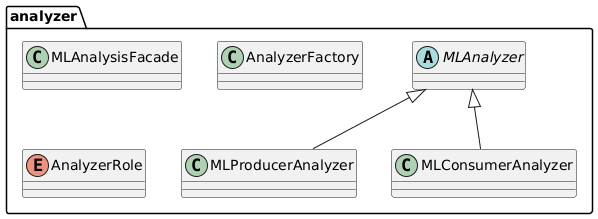
\includegraphics[width=0.8\linewidth]{pkg-analyzer.png}
  \caption{Package \pkgpath{modules/analyzer}}
  \label{fig:pkg-analyzer}
\end{figure}

\begin{itemize}
  \item \cls{MLAnalyzer} \emph{(astratta)}: classe base per tutti gli analyzer.
    Definisce il workflow comune per scansionare i progetti, applicare i filtri
    configurati, estrarre librerie e keyword ed esportare i risultati in CSV.
    Realizza il \textbf{Template Method}: i metodi di workflow sono fissi, le
    classi concrete specializzano solo \meth{check\_library}.

  \item \cls{MLProducerAnalyzer}: specializzazione per rilevare progetti che
    costruiscono o addestrano modelli ML. Applica i filtri di estensione e le
    strategie di keyword matching per identificare l'uso di API di training e
    di salvataggio modelli.

  \item \cls{MLConsumerAnalyzer}: specializzazione per identificare progetti che
    utilizzano modelli pre-addestrati. Applica le regole consumer sui file
    sorgente, con supporto opzionale della Rule 3 tramite il parametro
    \flag{rules\_3}.

  \item \cls{MLAnalysisFacade}: implementa il \textbf{Facade} che nasconde la
    complessit\`a del workflow dietro l'interfaccia semplificata
    \meth{run\_analysis(**kwargs)}. Coordina l'intera pipeline di analisi
    delegando alla factory la creazione degli analyzer e gestendo l'esecuzione
    end-to-end.

  \item \cls{AnalyzerFactory}: implementa un pattern \textbf{Factory-Registry}
    che permette la registrazione dinamica dei builder tramite il decoratore
    \meth{@register(role)} e l'istanziazione tramite
    \meth{create\_builder(role)}. Mantiene un registro interno delle classi
    builder associate ai vari ruoli di analisi.

  \item \cls{AnalyzerRole} \emph{(Enum)}: enumerazione che definisce i ruoli
    disponibili per gli analyzer ML. Nello stato iniziale i ruoli sono
    \code{PRODUCER} e \code{CONSUMER}.
\end{itemize}

\subsubsection{\pkgpath{modules/analyzer/builder} --- Costruzione configurata degli analyzer}

\begin{figure}[H]
  \centering
  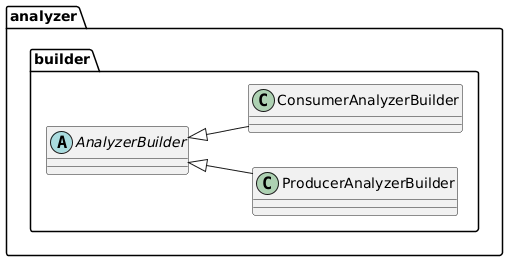
\includegraphics[width=0.72\linewidth]{pkg-analyzer-builder.png}
  \caption{Package \pkgpath{modules/analyzer/builder}}
  \label{fig:pkg-builder}
\end{figure}

\begin{itemize}
  \item \cls{AnalyzerBuilder} \emph{(astratta)}: implementa il \textbf{Builder}
    per assemblare istanze di \cls{MLAnalyzer} con configurazioni consistenti.
    Raccoglie passo dopo passo tutte le dipendenze richieste --- ruolo, filtri,
    strategie, dizionari --- e produce un analyzer completo solo quando la
    configurazione \`e valida. Centralizza la logica di setup, eliminando codice
    di inizializzazione duplicato e oggetti parzialmente configurati.

  \item \cls{ConsumerAnalyzerBuilder}: builder concreto pre-configurato per
    istanziare \cls{MLConsumerAnalyzer}. Registrato automaticamente tramite
    \meth{@register(AnalyzerRole.CONSUMER)}, configura di default il filtro
    \code{.py} e \cls{ExcludeTestFilesFilter}, i dizionari consumer/producer e
    la strategia \cls{DefaultKeywordMatcher}.

  \item \cls{ProducerAnalyzerBuilder}: builder concreto pre-configurato per
    istanziare \cls{MLProducerAnalyzer}. Registrato tramite
    \meth{@register(AnalyzerRole.PRODUCER)}, applica il filtro \code{.py}, il
    dizionario producer e la strategia \cls{DefaultKeywordMatcher} per rilevare
    le API di training.
\end{itemize}

\subsubsection{\pkgpath{modules/cloner} --- Acquisizione dei progetti}

\begin{figure}[H]
  \centering
  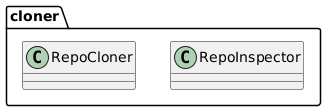
\includegraphics[width=0.5\linewidth]{pkg-cloner.png}
  \caption{Package \pkgpath{modules/cloner}}
  \label{fig:pkg-cloner}
\end{figure}

\begin{itemize}
  \item \cls{RepoCloner}: gestisce la clonazione di massa dei repository GitHub
    tramite \emph{shallow clone} paralleli con \cls{ThreadPoolExecutor}.
    Registra successi ed errori su file CSV (\file{cloned\_log.csv},
    \file{errors.csv}) per tracciare gli esiti del processo di acquisizione, e
    salta i repository gi\`a clonati rendendo le esecuzioni idempotenti.

  \item \cls{RepoInspector}: analizza i risultati del processo di clonazione
    verificando quali repository sono stati effettivamente clonati. Confronta il
    file CSV di log con il filesystem e genera report di riconciliazione
    (\file{not\_cloned\_repos.csv}, \file{effective\_repos.csv}).
\end{itemize}

\subsubsection{\pkgpath{modules/keyword\_extractor} --- Estrazione keyword e API}

\begin{figure}[H]
  \centering
  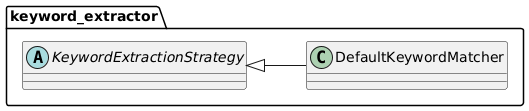
\includegraphics[width=0.72\linewidth]{pkg-keyword-extractor.png}
  \caption{Package \pkgpath{modules/keyword\_extractor}}
  \label{fig:pkg-keyword}
\end{figure}

\begin{itemize}
  \item \cls{KeywordExtractionStrategy} \emph{(astratta)}: definisce il
    contratto per l'estrazione di keyword dai file sorgente. Implementa lo
    \textbf{Strategy}, permettendo di sostituire dinamicamente l'algoritmo di
    matching senza modificare le classi analyzer.

  \item \cls{DefaultKeywordMatcher}: implementazione concreta dell'estrazione
    keyword mediante scansione riga per riga con pattern regex. Costruisce
    espressioni regolari case-insensitive gestendo i caratteri speciali (punti,
    parentesi) e il whitespace opzionale, restituendo le keyword trovate con il
    numero di riga corrispondente.
\end{itemize}

\subsubsection{\pkgpath{modules/library\_manager} --- Dizionari e import ML}

\begin{figure}[H]
  \centering
  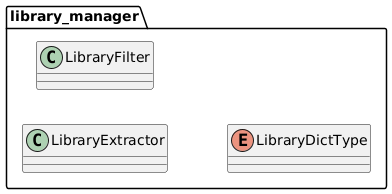
\includegraphics[width=0.6\linewidth]{pkg-library-manager.png}
  \caption{Package \pkgpath{modules/library\_manager}}
  \label{fig:pkg-library}
\end{figure}

\begin{itemize}
  \item \cls{LibraryExtractor}: utility per identificare gli statement di import
    nei file sorgente Python. Esegue matching testuale riga per riga su pattern
    \code{import} e \code{from...import}, estraendo i nomi delle librerie
    utilizzate nel codice.

  \item \cls{LibraryFilter}: fornisce metodi per caricare i dizionari di
    librerie ML da file CSV e filtrare quelle effettivamente utilizzate nei
    progetti. Confronta le librerie importate con quelle presenti nei dizionari
    consumer e producer.

  \item \cls{LibraryDictType} \emph{(Enum)}: enumerazione che identifica i tipi
    di dizionario disponibili (\code{CONSUMER}, \code{PRODUCER}) per
    categorizzare le librerie ML in base al loro utilizzo tipico.
\end{itemize}

\subsubsection{\pkgpath{modules/scanner} --- Filtraggio e scansione file}

\begin{figure}[H]
  \centering
  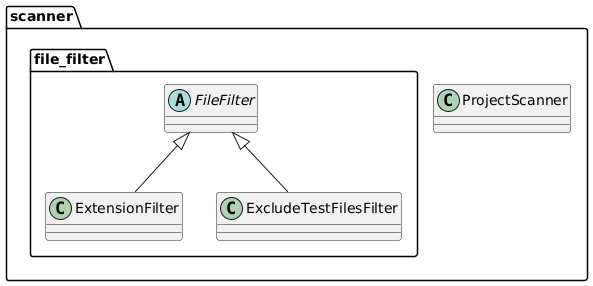
\includegraphics[width=0.8\linewidth]{pkg-scanner.png}
  \caption{Package \pkgpath{modules/scanner}}
  \label{fig:pkg-scanner}
\end{figure}

\begin{itemize}
  \item \cls{FileFilter} \emph{(astratta)}: classe base per implementare filtri
    di selezione dei file durante la scansione. Definisce il metodo
    \meth{accepts(file\_path)} che le classi concrete specializzano.

  \item \cls{ExtensionFilter}: accetta esclusivamente file con estensioni
    specifiche (ad es.\ \code{.py}, \code{.ipynb}), limitando l'analisi a
    determinati tipi di file sorgente.

  \item \cls{ExcludeTestFilesFilter}: scarta i file comunemente associati a
    testing, esempi, valutazioni o validazioni sulla base di pattern nel nome
    file. Implementa la Rule 4 dei Consumer, escludendo codice non
    rappresentativo dell'utilizzo reale.

  \item \cls{ProjectScanner}: coordina la scansione ricorsiva delle cartelle di
    progetto per raccogliere i file sorgente che soddisfano tutti i filtri
    configurati, applicandoli in sequenza.
\end{itemize}

\subsubsection{\pkgpath{modules/oracle} e \pkgpath{modules/utils} --- Validazione e logging}

\begin{figure}[H]
  \centering
  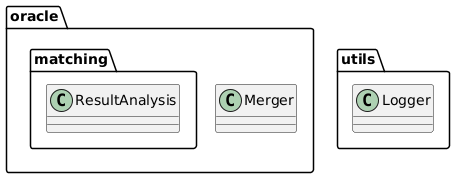
\includegraphics[width=0.68\linewidth]{pkg-oracle-utils.png}
  \caption{Package \pkgpath{modules/oracle} e \pkgpath{modules/utils}}
  \label{fig:pkg-oracle}
\end{figure}

\begin{itemize}
  \item \cls{Merger}: compara i risultati dell'analisi con un file oracolo di
    \emph{ground truth} e calcola le metriche di valutazione (Precision, Recall,
    F1-Score, Accuracy). Esporta falsi positivi e falsi negativi in file CSV
    separati per l'analisi degli errori.

  \item \cls{ResultAnalysis}: confronta i risultati ottenuti dai singoli
    progetti analizzati con il file oracolo di riferimento. Aggrega le metriche
    a livello di progetto ed esporta un report CSV con tutti i valori di
    performance per ogni repository.

  \item \meth{get\_logger()}: funzione factory che crea e restituisce
    un'istanza configurata di logger Python. Il logger \`e utilizzato
    trasversalmente da tutti i moduli per garantire tracciabilit\`a uniforme di
    operazioni, errori e performance del sistema.
\end{itemize}

\subsection{Flusso principale di utilizzo}
\label{sec:flusso}

Nello stato iniziale \baselineName{} \`e eseguibile tramite una pipeline avviata
dallo script \file{main.py}, che ne raccoglie i parametri di configurazione.

\begin{figure}[H]
  \centering
  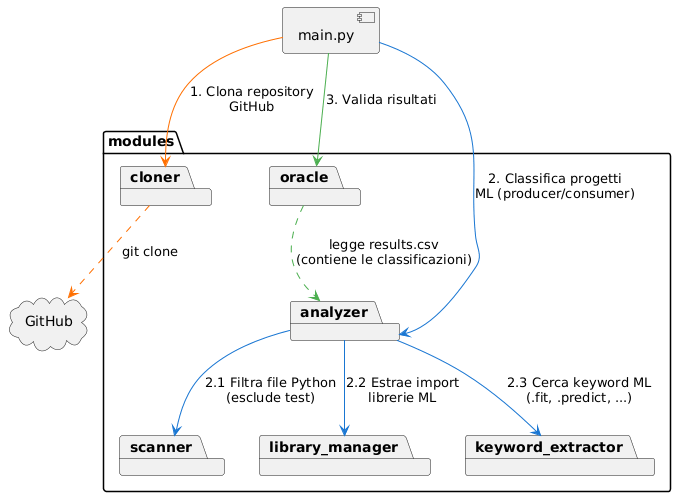
\includegraphics[width=0.86\linewidth]{component-flow.png}
  \caption{Flusso dei componenti a partire da \file{main.py}}
  \label{fig:component-flow}
\end{figure}

\subsubsection*{Step 1 --- Clonazione dei repository}

\cls{RepoCloner}:
\begin{enumerate}[nosep]
  \item legge un CSV con la lista dei progetti GitHub;
  \item clona in parallelo con \cls{ThreadPoolExecutor};
  \item genera la struttura \pkgpath{io/repos/<user>/<project>/...};
  \item \cls{RepoInspector} verifica la consistenza del file CSV con il
    filesystem.
\end{enumerate}

\subsubsection*{Step 2 --- Analisi ML (classificazione)}

\cls{MLAnalysisFacade} coordina un \cls{AnalyzerFactory} per costruire un
\cls{MLAnalyzer} specializzato; per ogni progetto:

\begin{enumerate}[nosep]
  \item filtra i file (ad es.\ \code{.py}) con \cls{ProjectScanner};
  \item estrae e filtra le librerie con \cls{LibraryExtractor} e
    \cls{LibraryFilter};
  \item trova keyword e API con \cls{DefaultKeywordMatcher};
  \item produce \file{results.csv} con una riga per evidenza rilevata
    (progetto, libreria, file, keyword/API, numero di riga).
\end{enumerate}

\begin{table}[H]
  \centering\small
  \caption{Struttura di una riga di \file{results.csv}}
  \label{tab:results-schema}
  \begin{tabularx}{\linewidth}{@{}L{2.6cm} L{1.9cm} L{2.1cm} L{2.4cm} L{1.7cm} Y@{}}
    \toprule
    \thead{ProjectName} & \thead{Is ML producer} & \thead{libraries} &
    \thead{where} & \thead{keyword} & \thead{line\_number}\\
    \midrule
    \code{user/repo-A} & Yes & \code{tensorflow} & \file{/model.py} &
    \code{.fit} & 45\\
    \bottomrule
  \end{tabularx}
\end{table}

\subsubsection*{Step 3 --- Validazione con oracolo (se attivato)}

\cls{Merger}:
\begin{enumerate}[nosep]
  \item calcola TP/FP/TN/FN e le metriche di classificazione;
  \item genera \file{false\_positives.csv} e \file{false\_negatives.csv}.
\end{enumerate}

\begin{figure}[H]
  \centering
  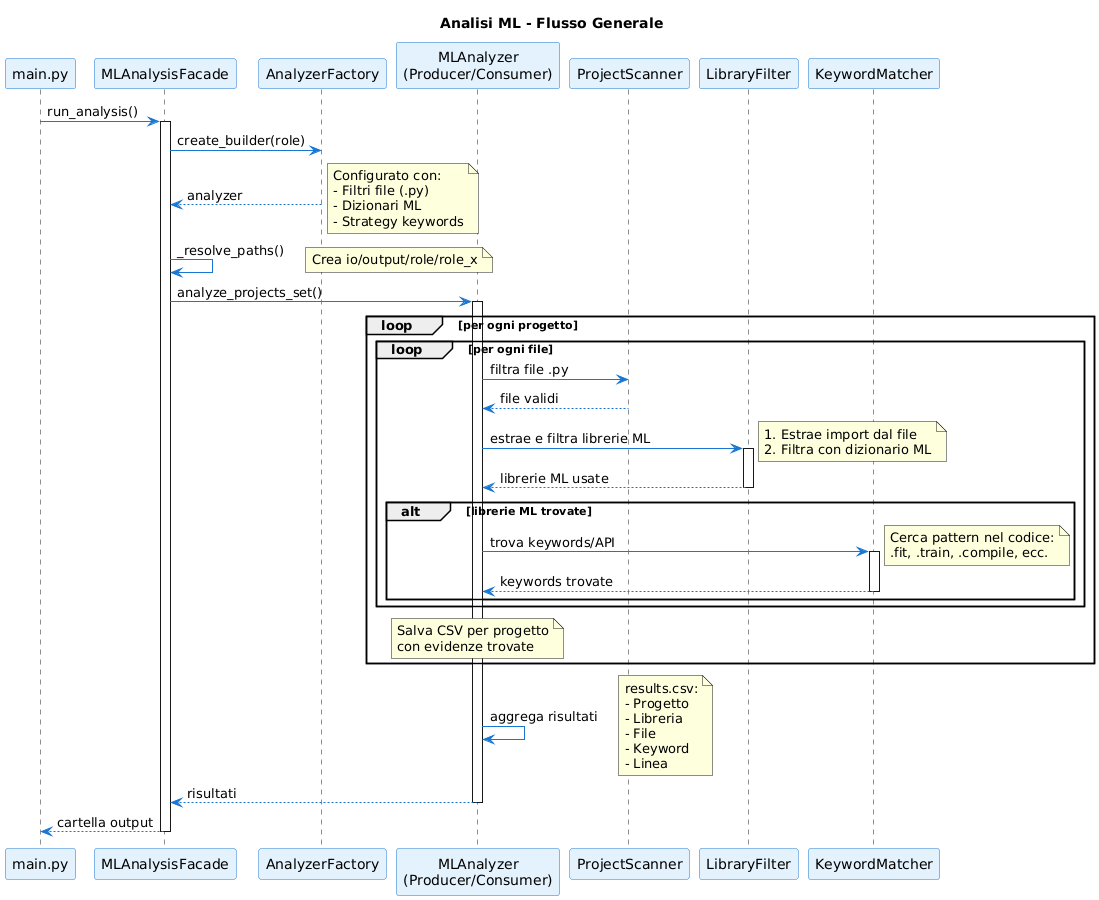
\includegraphics[width=\linewidth]{sequence-ml-analysis.png}
  \caption{Sequence diagram dello Step 2 --- Analisi ML}
  \label{fig:sequence-analysis}
\end{figure}

\subsection{Input e output}
\label{sec:io}

\subsubsection*{Input principali}

\begin{itemize}[nosep]
  \item CSV contenente la lista di repository GitHub, se si decide di utilizzare
    il cloner;
  \item cartella contenente i progetti da analizzare, se si decide di eseguire i
    soli step di analisi;
  \item \emph{knowledge base}: dizionari in formato \code{.csv} di librerie ML e
    API (training/inferenza), utilizzata per filtrare import e chiamate API.
\end{itemize}

\subsubsection*{Output principali}

\begin{itemize}[nosep]
  \item \textbf{Output cloner}: \file{cloned\_log.csv}, \file{errors.csv},
    \file{not\_cloned\_repos.csv}, \file{effective\_repos.csv}.
  \item \textbf{Output analisi}: \file{user\_repo\_ml\_producer.csv} o
    \file{user\_repo\_ml\_consumer.csv} per ogni singolo progetto classificato,
    e \file{results.csv} con i risultati uniti secondo lo schema di
    \cref{tab:results-schema}.
  \item \textbf{Output validazione}: metriche di Precision, Recall, F1 e
    Accuracy, con \file{false\_positives.csv} e \file{false\_negatives.csv}.
\end{itemize}

\subsection{Limiti dello stato iniziale}
\label{sec:limiti}

Lo stato appena descritto costituisce la \textbf{baseline} del lavoro. L'analisi
del sistema ne ha evidenziati tre limiti, riassunti in \cref{tab:limiti}: sono
questi a motivare, uno per uno, le tre Change Request definite nella
\cref{sec:cr}.

\begin{table}[H]
  \centering\small
  \caption{Limiti dello stato iniziale e Change Request corrispondente}
  \label{tab:limiti}
  \begin{tabularx}{\linewidth}{@{}C{1.1cm} L{4.2cm} Y C{1.1cm}@{}}
    \toprule
    \thead{ID} & \thead{Limite} & \thead{Situazione attuale (As-Is)} &
    \thead{CR}\\
    \midrule
    L1 & Assenza di indicatori di qualit\`a del codice &
      Il sistema produce output relativi a librerie, keyword e classificazione
      (ad es.\ \file{results.csv}), ma non calcola n\'e esporta alcuna metrica
      di complessit\`a o manutenibilit\`a a livello di progetto. & CR1\\
    L2 & Configurazione \emph{hard-coded} &
      I parametri della pipeline sono impostati direttamente nello script
      \file{main.py}: eseguire pi\`u run con configurazioni diverse richiede
      interventi manuali sul codice, e l'uso del tool resta orientato a utenti
      tecnici. & CR2\\
    L3 & Risultati consultabili solo come file &
      I risultati sono prodotti come CSV per run e per progetto, senza alcuna
      vista aggregata: l'interpretazione su pi\`u repository \`e demandata alla
      lettura manuale dei file. & CR3\\
    \bottomrule
  \end{tabularx}
\end{table}

Prima di intervenire su questi limiti, per\`o, la baseline \`e stata sottoposta
a verifica: \`e l'oggetto della sezione seguente.

% ===========================================================================
\section{Verifica della baseline: System Testing pre-modifica}
\label{sec:premod}

Prima dell'applicazione di qualunque Change Request il sistema \`e stato
sottoposto a una suite di \textbf{System Testing}. L'obiettivo \`e duplice:
verificare che la baseline si comporti come specificato e, soprattutto,
costruire una \textbf{base riutilizzabile} per il Regression Testing
post-modifica (\cref{sec:regression}).

\subsection{Scomposizione in casi d'uso}
\label{sec:usecases}

Per eseguire il system testing in modo pi\`u efficace e controllabile,
l'utilizzo del sistema \`e stato scomposto in due funzionalit\`a / casi d'uso
separati:

\begin{itemize}[nosep]
  \item \textbf{UC-1 (Analysis)}: analisi e classificazione di una directory
    locale contenente repository;
  \item \textbf{UC-2 (Cloning)}: clonazione di repository Git da una lista CSV.
\end{itemize}

\begin{keypoints}
\textbf{Nota.} L'analisi (UC-1) pu\`o essere eseguita \textbf{anche senza
cloning}, a condizione di disporre di una directory con repository gi\`a
presenti localmente. \`E questa indipendenza a rendere i due casi d'uso
testabili separatamente.
\end{keypoints}

\subsection{Tipologia e tecnica di testing}
\label{sec:catpart}

La tecnica scelta \`e il \textbf{testing funzionale / black-box}, che consente
di verificare il comportamento esterno del sistema rispetto ai requisiti
specificati, senza analizzarne l'implementazione interna.

Per la progettazione dei casi di test \`e stato adottato il metodo
\textbf{Category Partition}~\cite{ostrandbalcer}, una strategia che permette di:

\begin{itemize}[nosep]
  \item individuare i \textbf{parametri} di input e gli \textbf{oggetti
    dell'ambiente} rilevanti per ogni caso d'uso;
  \item suddividere ciascun parametro in \textbf{categorie} e \textbf{scelte}
    (classi di equivalenza);
  \item generare \textbf{test frame} validi, ciascuno rappresentante un insieme
    coerente di scelte;
  \item derivare da questi i \textbf{test case} eseguibili e i rispettivi
    \textbf{oracoli} (risultati attesi).
\end{itemize}

\`E la stessa tecnica adottata pi\`u avanti per il system testing delle nuove
funzionalit\`a (\cref{sec:st}), dove non viene ridescritta.

\subsection{Entry-point per l'esecuzione dei test: \file{main\_args.py}}
\label{sec:entrypoint}

Allo stato iniziale l'avvio era disponibile solo tramite \file{main.py}, ma
diversi parametri risultavano configurati tramite variabili \emph{hard-coded}
(limite L2 di \cref{tab:limiti}), rendendo poco pratico eseguire pi\`u scenari
in modo ripetibile senza modifiche manuali al codice.

Per questo motivo, per l'attivit\`a di system testing \`e stata introdotta una
variante dell'entry-point, denominata \file{main\_args.py}, invocabile da
terminale con argomenti CLI, cos\`i da selezionare i parametri necessari ai test
mantenendo invariato il codice sorgente.

\begin{lstlisting}[style=markshell,caption={Invocazione tipica usata dai test di sistema}]
python main_args.py --repository-path <dir> --analysis
python main_args.py --project-list <csv> --clone --clone-check
\end{lstlisting}

\subsection{UC-1 --- Analisi di una directory di repository}
\label{sec:uc1}

\begin{table}[H]
  \centering\small
  \caption{UC-1 --- Analysis}
  \label{tab:uc1}
  \begin{tabularx}{\linewidth}{@{}L{3.1cm} Y@{}}
    \toprule
    \thead{Descrizione} & L'utente esegue solo l'analisi su una directory locale
      contenente repository gi\`a disponibili, ottenendo i risultati in
      \pkgpath{io/output/}.\\
    \midrule
    \thead{Attori} & Utente (ricercatore)\\
    \midrule
    \thead{Entry condition} & \file{main\_args.py} disponibile; dipendenze
      installate; directory \flag{--repository-path} accessibile (per scenari
      ``success'').\\
    \midrule
    \thead{Exit condition} &
      \emph{Successo}: risultati salvati in \pkgpath{io/output/}.\newline
      \emph{Errore}: messaggio d'errore e assenza di output significativo.\\
    \midrule
    \thead{Flusso di eventi principale} &
      1. Invocazione con \flag{--repository-path} e \flag{--analysis}.\newline
      2. Validazione path.\newline
      3. Scansione e analisi dei repository.\newline
      4. Salvataggio output in \pkgpath{io/output/}.\\
    \bottomrule
  \end{tabularx}
\end{table}

\textbf{Parametri}: path della directory contenente i repository
(\flag{repository\_path}).

\textbf{Oggetti dell'ambiente}: filesystem, contenuto dei progetti appartenenti
alla directory analizzata.

\subsubsection{Categorie e scelte}

\begin{table}[H]
  \centering\small
  \caption{UC-1 --- Categorie e scelte}
  \label{tab:uc1-cat}
  \begin{tabularx}{\linewidth}{@{}L{3.4cm} L{1.4cm} L{4.3cm} Y@{}}
    \toprule
    \thead{Categoria} & \thead{ID} & \thead{Descrizione} &
    \thead{Propriet\`a / Vincoli}\\
    \midrule
    \multirow{2}{=}{Esistenza input directory}
      & ID1 & Directory non esiste & [Error]\\
      & ID2 & Directory esiste     & [property DirOk]\\
    \midrule
    \multirow{3}{=}{Contenuto directory}
      & CI0 & Directory vuota (0 progetti)  & [if DirOk] [property Empty]\\
      & CI1 & Directory con 1 progetto      & [if DirOk] [property NonEmpty]\\
      & CI2 & Directory con pi\`u progetti ($>1$) & [if DirOk] [property NonEmpty, MultiProject]\\
    \midrule
    \multirow{3}{=}{Cardinalit\`a Producer}
      & NP0 & 0 producer  & [if DirOk]\\
      & NP1 & 1 producer  & [if NonEmpty]\\
      & NP2 & 2+ producer & [if MultiProject] [Single]\\
    \midrule
    \multirow{3}{=}{Cardinalit\`a Consumer}
      & NC0 & 0 consumer  & [if DirOk]\\
      & NC1 & 1 consumer  & [if NonEmpty]\\
      & NC2 & 2+ consumer & [if MultiProject] [Single]\\
    \bottomrule
  \end{tabularx}
\end{table}

\subsubsection{Test Frame}

\begin{longtable}{@{}L{1.5cm} L{4.6cm} L{8.8cm}@{}}
  \caption{UC-1 --- Test frame}\label{tab:uc1-tf}\\
  \toprule
  \thead{ID} & \thead{Combinazioni (categorie/scelte)} &
  \thead{Oracolo (risultato atteso)}\\
  \midrule
  \endfirsthead
  \toprule
  \thead{ID} & \thead{Combinazioni (categorie/scelte)} &
  \thead{Oracolo (risultato atteso)}\\
  \midrule
  \endhead
  \bottomrule
  \endfoot
  TF1  & ID1                & Messaggio di errore ``Input folder not found''\\
  TF2  & ID2, CI0, NP0, NC0 & Nessun progetto classificato\\
  TF3  & ID2, CI1, NP0, NC0 & Progetto non classificato\\
  TF4  & ID2, CI1, NP1, NC0 & Progetto classificato ``Producer''\\
  TF5  & ID2, CI1, NP0, NC1 & Progetto classificato ``Consumer''\\
  TF6  & ID2, CI1, NP1, NC1 & Progetto classificato ``Producer + Consumer''\\
  TF7  & ID2, CI2, NP0, NC0 & Nessun progetto classificato\\
  TF8  & ID2, CI2, NP1, NC0 & Almeno un progetto classificato ``Producer''\\
  TF9  & ID2, CI2, NP0, NC1 & Almeno un progetto classificato ``Consumer''\\
  TF10 & ID2, CI2, NP1, NC1 & Almeno 1 ``Producer'' e 1 ``Consumer'', oppure 1 ``Producer+Consumer''\\
  TF11 & ID2, CI2, NP2, NC1 & 2+ progetti classificati ``Producer''\\
  TF12 & ID2, CI2, NP1, NC2 & 2+ progetti classificati ``Consumer''\\
\end{longtable}

\subsubsection{Test Case}

\begin{longtable}{@{}L{1.4cm} L{3.1cm} L{3.9cm} L{6.1cm}@{}}
  \caption{UC-1 --- Test case}\label{tab:uc1-tc}\\
  \toprule
  \thead{TC} & \thead{Input (\flag{repository\_path})} &
  \thead{Descrizione ambiente} & \thead{Oracolo}\\
  \midrule
  \endfirsthead
  \toprule
  \thead{TC} & \thead{Input (\flag{repository\_path})} &
  \thead{Descrizione ambiente} & \thead{Oracolo}\\
  \midrule
  \endhead
  \bottomrule
  \endfoot
  TC1  & \file{repo\_does\_not\_exist} & Directory inesistente & Messaggio ``Input folder not found''\\
  TC2  & \file{empty\_repo}  & Cartella vuota & Nessun progetto classificato\\
  TC3  & \file{test\_repos}  & 1 progetto senza librerie ML & Nessun progetto classificato\\
  TC4  & \file{test\_repos}  & 1 progetto con funzioni di training & Progetto classificato ``Producer''\\
  TC5  & \file{test\_repos}  & 1 progetto con funzioni di inferenza & Progetto classificato ``Consumer''\\
  TC6  & \file{test\_repos}  & 1 progetto con training e inferenza separati & Progetto classificato ``Producer + Consumer''\\
  TC7  & \file{test\_repos}  & Pi\`u progetti, nessuno ML & Nessun progetto classificato\\
  TC8  & \file{test\_repos}  & Pi\`u progetti, almeno uno con training & Almeno un progetto ``Producer''\\
  TC9  & \file{test\_repos}  & Pi\`u progetti, almeno uno con inferenza & Almeno un progetto ``Consumer''\\
  TC10 & \file{test\_repos}  & Pi\`u progetti con training e inferenza & Almeno un ``Producer'' e un ``Consumer''\\
  TC11 & \file{test\_repos}  & $\geq 2$ progetti con training & Almeno due ``Producer''\\
  TC12 & \file{test\_repos}  & $\geq 2$ progetti con inferenza & Almeno due ``Consumer''\\
\end{longtable}

\begin{keypoints}
\textbf{Implementazione.} I dodici test case sono implementati in
\file{test/system\_testing/analysis\_test/analysis\_test.py}; gli ambienti
descritti sopra corrispondono alle directory versionate sotto
\pkgpath{analysis\_test/test\_repos/} (TF3 \ldots TF12).
\end{keypoints}

\subsection{UC-2 --- Cloning (e verifica cloning) da lista CSV}
\label{sec:uc2}

\begin{table}[H]
  \centering\small
  \caption{UC-2 --- Cloning}
  \label{tab:uc2}
  \begin{tabularx}{\linewidth}{@{}L{3.1cm} Y@{}}
    \toprule
    \thead{Descrizione} & L'utente clona i repository elencati in un CSV e
      verifica gli esiti, salvando i repository in \pkgpath{io/repos/} e
      producendo log e report.\\
    \midrule
    \thead{Attori} & Utente (ricercatore)\\
    \midrule
    \thead{Entry condition} & \file{main\_args.py} disponibile; dipendenze
      installate; CSV disponibile (per gli scenari di successo); accesso a
      rete/Git; permessi di scrittura in \pkgpath{io/repos/}.\\
    \midrule
    \thead{Exit condition} &
      \emph{Successo}: repo clonati in \pkgpath{io/repos/} e report
      disponibili.\newline
      \emph{Errore}: messaggio d'errore e cloning non eseguito o parziale.\\
    \midrule
    \thead{Flusso di eventi principale} &
      1. Invocazione con \flag{--project-list}, \flag{--clone},
         \flag{--clone-check}.\newline
      2. Validazione CSV.\newline
      3. Clonazione repo in \pkgpath{io/repos/}.\newline
      4. Verifica cloning e report.\newline
      5. Terminazione.\\
    \bottomrule
  \end{tabularx}
\end{table}

\textbf{Parametri}: path del file CSV contenente l'elenco di repository
(\flag{project\_list\_path}).

\textbf{Oggetti dell'ambiente}: filesystem, contenuto del file CSV specificato.

\subsubsection{Categorie e scelte}

\begin{table}[H]
  \centering\small
  \caption{UC-2 --- Categorie e scelte}
  \label{tab:uc2-cat}
  \begin{tabularx}{\linewidth}{@{}L{3.4cm} L{1.4cm} L{4.6cm} Y@{}}
    \toprule
    \thead{Categoria} & \thead{ID} & \thead{Descrizione} & \thead{Vincoli}\\
    \midrule
    \multirow{2}{=}{Esistenza file CSV}
      & EF1 & File CSV non esiste & [Error]\\
      & EF2 & File CSV esiste     & [property file\_exists]\\
    \midrule
    \multirow{3}{=}{Contenuto CSV}
      & CC1 & CSV vuoto (solo header)        & [if file\_exists]\\
      & CC2 & CSV con 1 repository           & [if file\_exists]\\
      & CC3 & CSV con N repository ($>1$)    & [if file\_exists]\\
    \bottomrule
  \end{tabularx}
\end{table}

\subsubsection{Test Frame}

\begin{table}[H]
  \centering\small
  \caption{UC-2 --- Test frame}
  \label{tab:uc2-tf}
  \begin{tabularx}{\linewidth}{@{}L{1.5cm} L{3.6cm} Y@{}}
    \toprule
    \thead{ID} & \thead{Combinazioni} & \thead{Oracolo}\\
    \midrule
    TF1 & EF1      & Nessun repository clonato (errore: file inesistente)\\
    TF2 & EF2, CC1 & Nessun repository clonato (CSV vuoto)\\
    TF3 & EF2, CC2 & 1 repository clonato correttamente\\
    TF4 & EF2, CC3 & N repository clonati correttamente\\
    \bottomrule
  \end{tabularx}
\end{table}

\subsubsection{Test Case}

\begin{table}[H]
  \centering\small
  \caption{UC-2 --- Test case}
  \label{tab:uc2-tc}
  \begin{tabularx}{\linewidth}{@{}L{1.3cm} L{3.4cm} L{4.0cm} Y@{}}
    \toprule
    \thead{TC} & \thead{Input (\flag{project\_list\_path})} &
    \thead{Descrizione ambiente} & \thead{Oracolo}\\
    \midrule
    TC1 & \file{non-existent.csv} & File CSV inesistente &
      Messaggio ``Project list file not found''\\
    TC2 & \file{empty\_projects.csv} & File CSV vuoto &
      Nessun progetto clonato\\
    TC3 & \file{single\_project.csv} & Contiene \code{10up/classifai} &
      Il progetto \emph{classifai} viene clonato correttamente\\
    TC4 & \file{multi\_projects.csv} &
      Contiene \code{10up/classifai}, \code{2knal/Honesty},
      \code{5hirish/adam\_qas} &
      Tutti i repository vengono clonati correttamente\\
    \bottomrule
  \end{tabularx}
\end{table}

\begin{keypoints}
\textbf{Implementazione.} I quattro test case sono implementati in
\file{test/system\_testing/cloning\_test/cloning\_test.py}; i file CSV di input
sono versionati sotto \pkgpath{cloning\_test/test\_data/}.
\end{keypoints}

\subsection{Esito della suite pre-modifica}
\label{sec:premod-esito}

Il testing di sistema effettuato secondo la tecnica \textbf{Category
Partition} ha permesso di esplorare in modo sistematico tutte le combinazioni
significative dei parametri di input e dello stato degli oggetti dell'ambiente,
garantendo la copertura funzionale delle due principali funzionalit\`a del tool:
\emph{(i)} analisi e classificazione dei progetti ML ed \emph{(ii)} clonazione
dei repository da file CSV.

Complessivamente sono stati definiti, implementati ed eseguiti \textbf{16 test
case} --- 12 per UC-1 \emph{Analysis} e 4 per UC-2 \emph{Cloning} --- e
l'esecuzione \`e terminata \textbf{senza alcun fallimento}: tutti i test case
hanno soddisfatto gli oracoli attesi.

\begin{table}[H]
  \centering\small
  \caption{Esito della suite pre-modifica}
  \label{tab:premod-esito}
  \begin{tabularx}{0.75\linewidth}{@{}Y C{2.4cm} C{2.4cm}@{}}
    \toprule
    \thead{Caso d'uso} & \thead{Test case} & \thead{Esito}\\
    \midrule
    UC-1 Analysis & 12 & \tagok{12 pass}\\
    UC-2 Cloning  & 4  & \tagok{4 pass}\\
    \midrule
    \textbf{Totale} & \textbf{16} & \tagok{0 fallimenti}\\
    \bottomrule
  \end{tabularx}
\end{table}

Questa base di test viene riutilizzata \textbf{integralmente} come suite di
regressione nella \cref{sec:regression}, per verificare che le modifiche
introdotte dalle Change Request non compromettano il comportamento corretto del
sistema.

% ===========================================================================
\section{Le Change Request}
\label{sec:cr}

Verificata la baseline, l'evoluzione del sistema \`e stata definita attraverso
tre Change Request, ciascuna rivolta a uno dei limiti individuati in
\cref{tab:limiti}.

\begin{table}[H]
  \centering\small
  \caption{Le tre Change Request}
  \label{tab:cr-overview}
  \begin{tabularx}{\linewidth}{@{}C{1.0cm} L{3.6cm} Y L{3.3cm} C{1.7cm}@{}}
    \toprule
    \thead{ID} & \thead{Titolo} & \thead{Sintesi} & \thead{Tipo} &
    \thead{Stato}\\
    \midrule
    CR1 & Metriche di qualit\`a del codice &
      Introduzione del calcolo di metriche di qualit\`a tramite la libreria
      Radon: Cyclomatic Complexity (CC) e Maintainability Index (MI). &
      Enhancement (Additive + Perfective) & \tagok{Rilasciata}\\
    CR2 & GUI per configurazione ed esecuzione &
      Introduzione di una GUI (Tkinter) per configurare ed eseguire
      analisi e cloning senza modifiche manuali a script e variabili. &
      Enhancement (Additive) & \tagok{Rilasciata}\\
    CR3 & Dashboard di reportistica &
      Introduzione di una dashboard (matplotlib embedded nella GUI) con
      grafici e statistiche aggregate per run. &
      Enhancement (Additive + Perfective) & \tagok{Rilasciata}\\
    \bottomrule
  \end{tabularx}
\end{table}

Le tre modifiche non sono indipendenti: \textbf{CR2} sfrutta e visualizza le
informazioni introdotte da \textbf{CR1}, quando disponibili, mentre
\textbf{CR3} dipende logicamente sia da CR1 (dati delle metriche) sia da CR2
(contenitore UI e gestione delle run).

\begin{figure}[H]
  \centering
  \begin{tikzpicture}[
      node distance=1.1cm and 2.0cm,
      box/.style={draw=markDark, thick, rounded corners=3pt, fill=markBand,
                  minimum width=3.1cm, minimum height=1.0cm, align=center,
                  font=\small},
      dep/.style={-{Stealth[length=6pt]}, thick, draw=markDark}]
    \node[box] (cr1) {\textbf{CR1}\\Metriche CC/MI};
    \node[box, right=of cr1] (cr2) {\textbf{CR2}\\GUI};
    \node[box, right=of cr2] (cr3) {\textbf{CR3}\\Dashboard};
    \draw[dep] (cr1) -- node[above, font=\scriptsize\color{markMid}] {dati} (cr2);
    \draw[dep] (cr2) -- node[above, font=\scriptsize\color{markMid}] {contenitore UI} (cr3);
    \draw[dep] (cr1.south) to[out=-30, in=-150]
      node[below, font=\scriptsize\color{markMid}] {dati metriche} (cr3.south);
  \end{tikzpicture}
  \caption{Dipendenze logiche tra le Change Request}
  \label{fig:cr-deps}
\end{figure}

\subsection{Standard per la classificazione delle Change Request}
\label{sec:cr-standard}

Secondo lo standard \textbf{ISO/IEC/IEEE 14764:2022}~\cite{iso14764}, una
\textbf{Modification Request (MR)} \`e un item informativo che identifica e
descrive cambiamenti proposti al prodotto o servizio. Una MR pu\`o essere
classificata secondo lo schema di \cref{fig:mr-taxonomy}.

\begin{figure}[H]
  \centering
  \begin{tikzpicture}[
      level distance=1.4cm,
      root/.style={draw=markDark, very thick, fill=markBand,
                   rounded corners=2pt, font=\small\bfseries,
                   inner sep=5pt},
      mid/.style={draw=markDark, thick, fill=markBand,
                  rounded corners=2pt, font=\small, inner sep=5pt},
      leaf/.style={draw=markRule, thick, fill=white,
                   rounded corners=2pt, font=\footnotesize, inner sep=4pt},
      arrow/.style={-{Stealth[length=5pt]}, draw=markMid}]

    \node[root] (mr) at (0,0) {Modification request};

    \node[mid] (corr) at (-3.6,-1.6) {Correction};
    \node[mid] (enh)  at ( 3.6,-1.6) {Enhancement};

    \node[leaf] (corrective)  at (-6.4,-3.4) {Corrective};
    \node[leaf] (preventive)  at (-4.0,-3.4) {Preventive};
    \node[leaf] (adaptive)    at (-1.3,-3.4) {Adaptive};
    \node[leaf] (additive)    at ( 1.6,-3.4) {Additive};
    \node[leaf] (perfective)  at ( 4.6,-3.4) {Perfective};

    \draw[arrow] (mr) -- (corr);
    \draw[arrow] (mr) -- (enh);
    \draw[arrow] (corr) -- (corrective);
    \draw[arrow] (corr) -- (preventive);
    \draw[arrow] (corr) -- (adaptive);
    \draw[arrow] (enh)  -- (adaptive);
    \draw[arrow] (enh)  -- (additive);
    \draw[arrow] (enh)  -- (perfective);

    \node[font=\scriptsize\color{markMid}, anchor=east] at (-7.4,-1.6) {Classified};
    \node[font=\scriptsize\color{markMid}, anchor=east, align=right]
      at (-7.4,-3.4) {Types of\\maintenance};
  \end{tikzpicture}
  \caption{Classificazione di una Modification Request secondo
           ISO/IEC/IEEE 14764:2022~\cite{iso14764}}
  \label{fig:mr-taxonomy}
\end{figure}

In particolare, una \textbf{Correction} \`e un cambiamento che risolve un
problema e colma un gap per rendere il software operativo rispetto ai requisiti
operativi definiti. Un \textbf{Enhancement} \`e un cambiamento che implementa un
\textbf{nuovo requisito}; lo standard precisa che un enhancement \emph{non} \`e
una correction.

Dopo la classificazione principale, la MR pu\`o essere identificata anche con
una \emph{tipologia di manutenzione}:

\begin{itemize}
  \item \textbf{Adaptive maintenance} (collegabile a correction ed
    enhancement): modifica per mantenere il prodotto usabile in un ambiente
    cambiato o in costante cambiamento;
  \item \textbf{Additive maintenance} (enhancement): modifica post-delivery per
    \textbf{aggiungere funzionalit\`a o feature};
  \item \textbf{Perfective maintenance} (enhancement): modifica per fornire
    miglioramenti agli utenti in termini di comprensibilit\`a e informazione,
    e/o per migliorare performance, manutenibilit\`a o altri attributi.
\end{itemize}

Ogni CR riporta di seguito la \textbf{classificazione} (Enhancement o
Correction) e la \textbf{tipologia di manutenzione} con una breve motivazione.

\subsection{CR1 --- Metriche di qualit\`a del codice (Radon)}
\label{sec:cr1}

\subsubsection*{Motivazione}

Nella versione attuale, \baselineName{} produce risultati di classificazione ML
(Producer/Consumer) ma non include indicatori quantitativi di qualit\`a del
codice del progetto (limite L1 di \cref{tab:limiti}). In contesti di analisi su
dataset di repository, poter associare ai risultati anche misure come
complessit\`a e manutenibilit\`a facilita:

\begin{itemize}[nosep]
  \item l'interpretazione dei risultati;
  \item il confronto tra repository;
  \item la selezione di progetti ``pi\`u manutenibili'' per analisi successive.
\end{itemize}

\subsubsection*{Situazione desiderata (To-Be)}

Integrare nella pipeline il calcolo di metriche tramite \textbf{Radon}, in
particolare:

\begin{itemize}[nosep]
  \item \textbf{Cyclomatic Complexity (CC)}~\cite{mccabe};
  \item \textbf{Maintainability Index (MI)}~\cite{colemanoman}.
\end{itemize}

Le metriche devono essere calcolate sui file sorgente analizzati e aggregate a
livello di progetto.

\subsubsection*{Descrizione della modifica}

\begin{itemize}
  \item Durante l'analisi dei file, oltre all'estrazione di librerie e keyword,
    il sistema calcola CC e MI.
  \item I valori delle metriche vengono raccolti e aggregati a livello di
    progetto secondo le formule di \cref{eq:cc,eq:mi}: la CC \`e
    calcolata per ogni blocco di codice presente nei file Python e mediata
    aritmeticamente su tutti i blocchi; l'MI \`e calcolato per ciascun file
    Python e poi mediato in modo \textbf{pesato sullo SLOC} di ogni file,
    ottenendo una media complessiva rappresentativa dell'intero progetto.
  \item Le metriche vengono salvate in output in modo consultabile e allineato
    alla run corrente.
\end{itemize}

\begin{align}
  \overline{CC}_{p} &= \frac{1}{|B_p|}\sum_{b \in B_p} CC(b)
  \label{eq:cc}\\[4pt]
  \overline{MI}_{p} &=
    \frac{\sum_{f \in F_p} MI(f)\cdot SLOC(f)}{\sum_{f \in F_p} SLOC(f)}
  \label{eq:mi}
\end{align}

dove $B_p$ \`e l'insieme dei blocchi di codice del progetto $p$ e $F_p$
l'insieme dei suoi file Python con $SLOC(f) > 0$.

\begin{keypoints}
\textbf{Perch\'e l'MI \`e pesato e la CC no.} La CC \`e gi\`a una misura per
blocco, quindi la media aritmetica sui blocchi \`e la sua aggregazione naturale.
L'MI \`e invece definito per file: pesarlo sullo SLOC evita che un file di
poche righe con MI molto alto o molto basso domini il valore di progetto.
\end{keypoints}

\subsubsection*{Classificazione e tipologia di manutenzione}

\begin{table}[H]
  \centering\small
  \caption{CR1 --- Classificazione}
  \label{tab:cr1-class}
  \begin{tabularx}{\linewidth}{@{}L{3.3cm} Y@{}}
    \toprule
    \thead{Classificazione} & \textbf{Enhancement}\\
    \midrule
    \thead{Additive} & Aggiunge una nuova feature (calcolo e salvataggio di
      CC/MI) al tool.\\
    \midrule
    \thead{Perfective} & Arricchisce l'output con informazioni aggiuntive (CC e
      MI) che rendono l'analisi pi\`u completa, interpretabile e utile per
      l'utente.\\
    \bottomrule
  \end{tabularx}
\end{table}

\subsection{CR2 --- GUI per configurazione ed esecuzione analisi}
\label{sec:cr2}

\subsubsection*{Motivazione}

L'uso del tool nella situazione attuale richiede interventi manuali su parametri
\emph{hard-coded} nello script \file{main.py} (limite L2 di \cref{tab:limiti}),
rendendo meno pratico eseguire velocemente pi\`u run con configurazioni diverse
e limitando l'accesso ad utenti non tecnici.

\subsubsection*{Situazione desiderata (To-Be)}

Introdurre una GUI (Tkinter) che consenta di:

\begin{itemize}[nosep]
  \item selezionare facilmente gli input (directory locale oppure CSV per il
    cloning);
  \item configurare i parametri di analisi (ruolo Producer/Consumer, opzioni
    regole, attivazione metriche);
  \item avviare l'analisi tramite un pulsante;
  \item consultare i risultati direttamente dall'interfaccia.
\end{itemize}

\subsubsection*{Descrizione della modifica}

La GUI organizza l'utilizzo del tool come un flusso guidato:

\begin{enumerate}
  \item \textbf{Input selection}: scelta della sorgente (cartella locale o
    cloning da CSV).
  \item \textbf{Configuration}: impostazione dei parametri principali (ruolo,
    regole, numero di repo se cloning, abilitazione metriche).
  \item \textbf{Execution}: avvio della run \textbf{senza bloccare
    l'interfaccia}, tramite gestione asincrona su thread separato.
  \item \textbf{Results}: visualizzazione dei file prodotti e dei contenuti
    principali (tabella o viewer integrato).
\end{enumerate}

\subsubsection*{Classificazione e tipologia di manutenzione}

\begin{table}[H]
  \centering\small
  \caption{CR2 --- Classificazione}
  \label{tab:cr2-class}
  \begin{tabularx}{\linewidth}{@{}L{3.3cm} Y@{}}
    \toprule
    \thead{Classificazione} & \textbf{Enhancement}\\
    \midrule
    \thead{Additive} & Aggiunge una nuova feature (GUI) per configurare ed
      eseguire il tool e per consultare i risultati, estendendo l'uso del
      sistema senza modificarne l'obiettivo funzionale principale.\\
    \bottomrule
  \end{tabularx}
\end{table}

\subsection{CR3 --- Dashboard di reportistica integrata nella GUI}
\label{sec:cr3}

\subsubsection*{Motivazione}

Nella versione attuale i risultati sono principalmente consultabili tramite file
CSV (limite L3 di \cref{tab:limiti}). Per analisi su pi\`u repository \`e utile
una vista aggregata che fornisca \emph{insight} rapidi e confrontabili, evitando
l'interpretazione manuale dei file.

\subsubsection*{Situazione desiderata (To-Be)}

Aggiungere una sezione ``Dashboard'' nella GUI con grafici (matplotlib
integrato) e statistiche aggregate per run.

\subsubsection*{Descrizione della modifica}

Dopo l'esecuzione di una run, la GUI deve poter costruire una dashboard basata
sugli output generati (CSV di risultati e metriche). La dashboard \`e pensata
come una vista di sintesi per dataset di repository.

\begin{table}[H]
  \centering\small
  \caption{CR3 --- Viste previste nella dashboard}
  \label{tab:cr3-views}
  \begin{tabularx}{\linewidth}{@{}L{4.6cm} Y@{}}
    \toprule
    \thead{Vista} & \thead{Contenuto}\\
    \midrule
    Analysis Overview & Numero e percentuale di progetti classificati come
      Producer, Consumer e Producer \& Consumer.\\
    Code Quality Metrics Overview & Riepilogo delle metriche introdotte da CR1
      (CC e MI medi).\\
    Top ML Keywords & Top 10 delle keyword ML (di training o inferenza) pi\`u
      rilevate per i risultati analizzati, con conteggio delle occorrenze.\\
    \bottomrule
  \end{tabularx}
\end{table}

\subsubsection*{Classificazione e tipologia di manutenzione}

\begin{table}[H]
  \centering\small
  \caption{CR3 --- Classificazione}
  \label{tab:cr3-class}
  \begin{tabularx}{\linewidth}{@{}L{3.3cm} Y@{}}
    \toprule
    \thead{Classificazione} & \textbf{Enhancement}\\
    \midrule
    \thead{Additive} & Aggiunge una nuova feature di reportistica.\\
    \midrule
    \thead{Perfective} & Fornisce miglioramenti informativi per gli utenti
      (viste aggregate, insight e visualizzazioni), migliorando la fruibilit\`a
      dei risultati della run e supportando valutazioni complessive su dataset
      di repository.\\
    \bottomrule
  \end{tabularx}
\end{table}

% ===========================================================================
\section{Master Test Plan}
\label{sec:mtp}

Definite le modifiche, prima di implementarle \`e stato fissato l'approccio di
testing con cui verificarle. Il presente \textbf{Master Test Plan} vale per
\projectName{} nel suo complesso --- funzionalit\`a della baseline ed evoluzioni
introdotte dalle tre Change Request --- e definisce:

\begin{itemize}[nosep]
  \item i livelli di test previsti (unit\`a, integrazione, sistema);
  \item le tecniche utilizzate;
  \item i componenti su cui concentrare lo sforzo di verifica;
  \item un criterio di copertura strutturale per le parti testate in white-box.
\end{itemize}

\subsection{Strategia di testing}
\label{sec:mtp-strategia}

La strategia \`e articolata su tre livelli, riassunti in
\cref{tab:mtp-strategia}.

\begin{table}[H]
  \centering\small
  \caption{Livelli di test, tecniche e criteri di selezione}
  \label{tab:mtp-strategia}
  \begin{tabularx}{\linewidth}{@{}L{3.2cm} L{2.3cm} L{3.0cm} Y@{}}
    \toprule
    \thead{Livello} & \thead{Tecnica} & \thead{Selezione input} &
    \thead{Dipendenze}\\
    \midrule
    Basic Unit Testing   & White-box & CFG dei metodi target &
      Mockate dove necessario\\
    Integration Testing  & White-box & CFG dei metodi target &
      Reali (nessun mock)\\
    System Testing       & Black-box & Category Partition &
      Sistema completo via CLI/GUI\\
    \bottomrule
  \end{tabularx}
\end{table}

\subsubsection{Basic Unit Testing (white-box)}
\label{sec:mtp-unit}

Verr\`a effettuato un \textbf{basic unit testing} focalizzato sui \textbf{metodi}
delle classi selezionate, con l'obiettivo di verificare la logica interna dei
rami principali. Quando necessario, le dipendenze verranno \textbf{mockate} per
isolare il metodo sotto test e controllare lo stato dell'ambiente (ad es.\
filesystem, servizi del tool).

La progettazione dei test avverr\`a in modalit\`a \textbf{white-box}: per
ciascun metodo target verr\`a costruito il relativo \textbf{Control Flow Graph
(CFG)} tramite uno script Python basato su \textbf{AST}. A partire dal CFG
verranno individuati i percorsi che coprono il maggior numero di branch e
verranno scelti gli input in grado di attivarli. I percorsi selezionati verranno
poi implementati come casi di test.

\subsubsection{Integration Testing (white-box)}
\label{sec:mtp-integration}

Verr\`a eseguito anche \textbf{integration testing} sui componenti scelti, per
verificare le interazioni tra classi e servizi senza isolare artificialmente il
comportamento. In questa fase \textbf{non verranno mockate le dipendenze}: i
test utilizzeranno interazioni reali (filesystem reale o temporaneo, servizi del
tool).

Anche qui la selezione dei test verr\`a guidata dal CFG, con l'obiettivo di
coprire i branch pi\`u significativi dei metodi di interesse.

\subsubsection{System Testing (black-box, Category Partition)}
\label{sec:mtp-system}

Il \textbf{system testing} verr\`a condotto in modalit\`a \textbf{black-box}
progettando i casi di test tramite \textbf{Category
Partition}~\cite{ostrandbalcer}, con il procedimento gi\`a descritto in
\cref{sec:catpart}: la definizione delle categorie e delle scelte riguarder\`a i
parametri di input e lo stato dell'ambiente, che insieme agli oracoli saranno
ricavati dalle specifiche delle funzionalit\`a del sistema espresse in forma di
casi d'uso.

I test di sistema saranno pianificati:

\begin{itemize}[nosep]
  \item sul \textbf{sistema pre-modifica}, cos\`i da ottenere una suite
    riutilizzabile per \textbf{regressione} post-CR (\cref{sec:premod});
  \item sulle funzionalit\`a introdotte da \textbf{CR1--CR3}, con casi dedicati
    per ciascuna nuova feature (\cref{sec:st}).
\end{itemize}

Per favorire ripetibilit\`a ed evitare modifiche manuali a parametri
\emph{hard-coded}, dove opportuno l'esecuzione dei test di sistema verr\`a
effettuata tramite \file{main\_args.py} con pochi flag essenziali e valori di
default invariati (ad es.\ analisi su directory o cloning da CSV).

\subsection{Componenti incluse, componenti escluse e coverage}
\label{sec:mtp-componenti}

\subsubsection{Componenti incluse}
\label{sec:mtp-incluse}

\textbf{Unit testing} (basic, sui metodi):

\begin{itemize}[nosep]
  \item tutti i metodi del sistema che saranno \textbf{modificati dalla CR1};
  \item metodi delle classi \textbf{Service} della GUI, responsabili
    dell'interfacciamento tra Controller e servizi del sistema o filesystem.
\end{itemize}

\textbf{Integration testing}:

\begin{itemize}[nosep]
  \item gli stessi metodi scelti per l'unit testing;
  \item metodi della classe \textbf{Controller} della GUI, per verificare la
    logica di orchestrazione tra componenti grafiche e classi Service.
\end{itemize}

\begin{table}[H]
  \centering\small
  \caption{Componenti target del testing white-box}
  \label{tab:mtp-target}
  \begin{tabularx}{\linewidth}{@{}L{5.7cm} C{1.6cm} C{2.1cm} Y@{}}
    \toprule
    \thead{Componente} & \thead{Unit} & \thead{Integration} & \thead{CR}\\
    \midrule
    \pkgpath{modules/analyzer/ml\_analyzer.py} & \checkmark & \checkmark & CR1\\
    \pkgpath{gui/services/pipeline\_service.py} & \checkmark & \checkmark & CR2\\
    \pkgpath{gui/services/output\_reader.py} & \checkmark & \checkmark & CR2/CR3\\
    \pkgpath{gui/controller.py} & --- & \checkmark & CR2/CR3\\
    \bottomrule
  \end{tabularx}
\end{table}

\subsubsection{Componenti escluse}
\label{sec:mtp-escluse}

Le classi \textbf{View} della GUI verranno escluse dal testing white-box, poich\'e
si occupano prevalentemente di \textbf{logica di presentazione} (layout,
rendering) e non contengono logica applicativa core; lo sforzo di verifica viene
quindi concentrato su Controller, Service e sui componenti di analisi
modificati.

\begin{keypoints}
Le View restano comunque verificate \textbf{indirettamente} a livello di
sistema: i test black-box della CR2 e della CR3 pilotano l'interfaccia reale e
ne osservano gli effetti, quindi un difetto di presentazione che alteri il
comportamento osservabile viene rilevato.
\end{keypoints}

\subsubsection{Coverage}
\label{sec:mtp-coverage}

Per unit e integration testing verr\`a adottato un obiettivo di
$\geq \mathbf{80\%}$ \textbf{di branch coverage} sulle classi di interesse del
testing. La copertura verr\`a misurata con \textbf{pytest-cov}~\cite{pytestcov} e
calcolata \textbf{solo} sul sottoinsieme di componenti target elencato in
\cref{tab:mtp-target}.

\begin{lstlisting}[style=markshell,caption={Comando di misura della branch coverage}]
python -m pytest test/unit_testing \
  --cov=modules.analyzer.ml_analyzer \
  --cov=gui.services \
  --cov-branch --cov-report=term --cov-report=html
\end{lstlisting}

% ===========================================================================
\section{Impact Analysis}
\label{sec:ia}

Prima di implementare le Change Request \`e stato stimato il loro impatto sui
componenti esistenti. La sezione riporta, per ciascuna CR, il metodo adottato,
gli insiemi di impatto previsti e --- a valle dell'implementazione --- il
confronto con l'impatto effettivamente osservato.

\subsection{Metodo adottato e scelta degli SLO}
\label{sec:ia-metodo}

In assenza di artefatti di requisiti e design (ad es.\ SRS, diagrammi UML
aggiornati), l'Impact Analysis viene condotta sugli artefatti disponibili --- il
codice sorgente --- usando \emph{traceability} interna (vertical traceability) e
relazioni di dipendenza tra componenti.

Il riferimento teorico utilizzato~\cite{tripathynaik} introduce gli \textbf{SLO
(Software Life-cycle Objects)} come oggetti che possono variare di
granularit\`a. Nel nostro contesto, per mantenere una granularit\`a uniforme e
compatibile con un'analisi call-graph-based in ambiente OO, si assumono come SLO
i \textbf{metodi} del sistema software.

Le due CR che introducono l'interfaccia grafica sono state progettate in modo da
non toccare il core, e per questo richiedono un'analisi diversa da quella della
CR1: le due situazioni sono trattate separatamente nelle
\cref{sec:ia-cr1,sec:ia-cr23}.

\subsection{CR1 --- Metriche di qualit\`a del codice}
\label{sec:ia-cr1}

La CR1 introduce un'estensione funzionale al core: integrare il calcolo di
metriche di qualit\`a del codice (Radon~\cite{radon}), in particolare
\textbf{Cyclomatic Complexity (CC)}~\cite{mccabe} e \textbf{Maintainability
Index (MI)}~\cite{colemanoman}, calcolate sui file sorgente analizzati e
aggregate a livello di progetto secondo \cref{eq:cc,eq:mi}, con salvataggio dei
risultati in output allineato alla run corrente.

\subsubsection{Starting Impact Set (SIS)}
\label{sec:ia-cr1-sis}

Sulla base dell'analisi del sistema (\cref{sec:baseline}) e del contenuto della
CR1, vengono identificati come \emph{core methods} da modificare i tre metodi
``template'' della classe \cls{MLAnalyzer}, responsabili del workflow principale
di analisi:

\begin{equation*}
  \SIS = \Big\{
    \begin{array}{l}
      \meth{MLAnalyzer.analyze\_single\_file},\\
      \meth{MLAnalyzer.analyze\_project},\\
      \meth{MLAnalyzer.analyze\_projects\_set}
    \end{array}
  \Big\}
  \qquad |\SIS| = 3
\end{equation*}

\subsubsection{Candidate Impact Set (CIS): costruzione del call graph}
\label{sec:ia-cr1-cis}

La modifica dei metodi core di \cls{MLAnalyzer} pu\`o propagarsi:

\begin{itemize}[nosep]
  \item verso i \textbf{callee} (fan-out): nuove dipendenze invocate per
    calcolare CC/MI e salvarle;
  \item verso i \textbf{caller} (fan-in): eventuali adattamenti dovuti a
    variazioni di ritorni o dati prodotti, o a step aggiunti alla pipeline.
\end{itemize}

Per questo motivo si costruisce un sottografo includendo sia fan-out sia fan-in,
cos\`i da ottenere una stima \textbf{prudenziale} dei candidati al cambiamento.
La procedura adottata \`e:

\begin{enumerate}
  \item \textbf{Seeding}: inizializzazione dei nodi del grafo con gli SLO del
    SIS.
  \item \textbf{Espansione fan-out}: aggiunta iterativa dei metodi chiamati
    (callee) dai nodi correnti.
  \item \textbf{Espansione fan-in}: aggiunta iterativa dei metodi chiamanti
    (caller) che invocano i nodi correnti.
  \item \textbf{Arresto}: terminazione quando non emergono nuovi nodi interni al
    sistema.
  \item \textbf{Filtraggio}: esclusione di nodi esterni (librerie di terze parti
    o built-in) per mantenere il grafo sugli SLO del sistema.
\end{enumerate}

Il risultato \`e un sottografo statico che rappresenta una
\textbf{sovra-approssimazione} dei possibili impatti.

\begin{figure}[H]
  \centering
  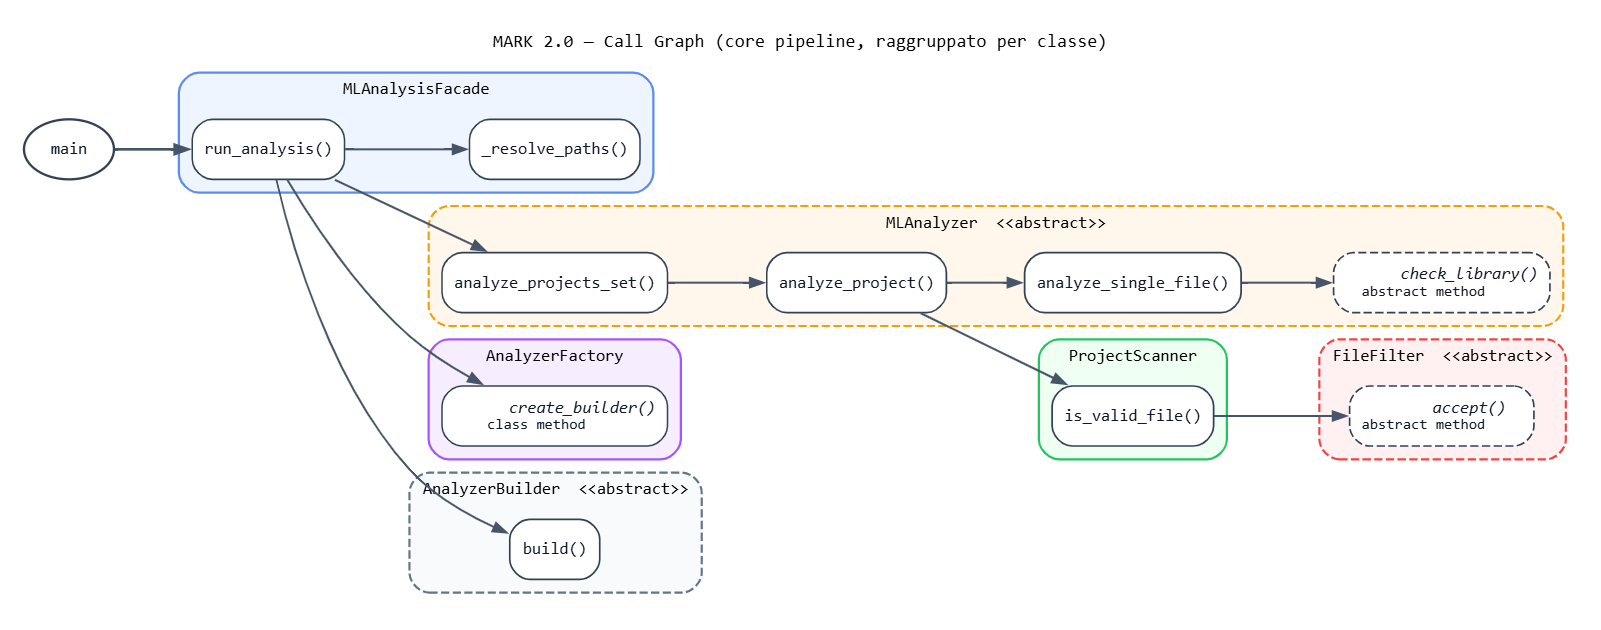
\includegraphics[width=\linewidth]{call-graph-core.png}
  \caption{Call graph della core pipeline di \baselineName{}, raggruppato per
           classe}
  \label{fig:call-graph}
\end{figure}

A partire dai tre metodi del SIS, il sottografo ricostruito include:

\begin{itemize}[nosep]
  \item l'entry-point della pipeline (\meth{main}), che invoca il Facade;
  \item \meth{MLAnalysisFacade.run\_analysis}, che orchestra l'analisi e attiva
    factory e builder;
  \item i metodi di costruzione
    (\meth{AnalyzerFactory.create\_builder}, \meth{AnalyzerBuilder.build});
  \item i metodi di workflow dell'analyzer
    (\meth{analyze\_projects\_set} $\rightarrow$ \meth{analyze\_project}
    $\rightarrow$ \meth{analyze\_single\_file});
  \item i metodi ausiliari chiamati nel workflow (validazione file e filtraggio;
    metodo astratto \meth{check\_library}).
\end{itemize}

\subsubsection{Valutazione incrementale dei nodi}
\label{sec:ia-cr1-valutazione}

Il call graph costruito produce un insieme di nodi raggiungibili dai metodi del
SIS e/o che li raggiungono: tale insieme \`e un \textbf{superset} di possibili
impatti. Tuttavia, la CR1 \`e specifica (aggiunta di CC/MI e relativo
salvataggio e aggregazione), quindi non tutti i nodi raggiungibili sono
necessariamente da modificare.

Per rendere l'Impact Analysis aderente alla definizione di CIS --- ``insieme
potenzialmente affetto'' ma non arbitrariamente esteso --- si introduce un passo
incrementale:

\begin{enumerate}[nosep]
  \item per ciascun nodo del sottografo si valuta se la CR pu\`o richiedere
    modifica \textbf{diretta} del comportamento, dei dati prodotti o consumati, o
    dell'orchestrazione in cui il nodo \`e coinvolto;
  \item se la pertinenza \`e nulla o trascurabile, il nodo viene escluso dal CIS.
\end{enumerate}

La valutazione dei componenti emersi \`e riportata in \cref{tab:ia-valutazione}.

\begin{longtable}{@{}L{6.0cm} C{1.3cm} L{7.4cm}@{}}
  \caption{Valutazione incrementale dei nodi del call graph}
  \label{tab:ia-valutazione}\\
  \toprule
  \thead{Nodo} & \thead{Esito} & \thead{Motivazione}\\
  \midrule
  \endfirsthead
  \toprule
  \thead{Nodo} & \thead{Esito} & \thead{Motivazione}\\
  \midrule
  \endhead
  \bottomrule
  \endfoot
  \meth{main} (entry-point) & \In &
    Potrebbe essere necessario per introdurre un nuovo flag o step nella
    pipeline.\\
  \meth{MLAnalysisFacade.run\_analysis} & \In &
    L'introduzione di un nuovo ruolo di analisi pu\`o richiedere gestione
    specifica di output/directory e corretta attivazione della build.\\
  \meth{MLAnalysisFacade.\_resolve\_paths} & \Out &
    Gestisce la risoluzione dei path dei dizionari ML e la creazione della
    cartella di output principale; non \`e necessaria per CR1.\\
  \meth{AnalyzerFactory.create\_builder} & \In &
    Candidato prudenziale: pu\`o risultare necessario per introdurre o
    risolvere il nuovo ruolo \code{METRICS} (potr\`a diventare FPIS se
    l'estensione avviene senza modifiche alla factory).\\
  \meth{AnalyzerBuilder.build} (astratto) & \In &
    Candidato prudenziale nel caso siano necessarie dipendenze o
    configurazioni diverse per la costruzione del nuovo analyzer.\\
  \meth{ProjectScanner.is\_valid\_file} / \meth{FileFilter.accept} & \Out &
    CR1 non modifica i criteri di selezione dei file; si riusano invariati i
    file gi\`a analizzati.\\
  \meth{MLAnalyzer.check\_library} (astratto) & \Out &
    La logica librerie/keyword non viene modificata; tuttavia CR1 richiede una
    nuova classe concreta che implementi \meth{check\_library} per il ruolo
    metrics (ad es.\ restituendo liste vuote). L'impatto \`e quindi sulla nuova
    implementazione concreta, non sul metodo astratto.\\
  \cls{AnalyzerRole} (Enum) & \In &
    Necessario per introdurre il nuovo ruolo \code{METRICS}.\\
\end{longtable}

\subsubsection*{Componenti da aggiungere}

Si prevede l'introduzione dei seguenti elementi:

\begin{itemize}[nosep]
  \item \cls{MLMetricsAnalyzer}: classe concreta di \cls{MLAnalyzer} che esegue
    l'override di \meth{check\_library} restituendo liste vuote, in quanto non
    interessa l'estrazione di librerie o keyword;
  \item \meth{MLAnalyzer.\_save\_metrics\_csv}: metodo per salvare i CSV
    relativi alle metriche;
  \item \cls{MetricsAnalyzerBuilder}: classe concreta di \cls{AnalyzerBuilder},
    costruttore di \cls{MLMetricsAnalyzer} richiamato dal Facade.
\end{itemize}

\subsubsection*{File e cartelle di output impattate}

\begin{itemize}[nosep]
  \item Cartella \pkgpath{logs}: i file \file{.log} potrebbero essere arricchiti
    con nuove informazioni di log generate dal nuovo step introdotto.
  \item Cartella \pkgpath{output}: potr\`a essere modificata dalla creazione di
    una nuova cartella risultati \pkgpath{metrics}, con una sottocartella per
    ogni run (\pkgpath{metrics\_<num\_run>}) e file \file{.csv} contenenti le
    metriche calcolate.
\end{itemize}

\subsubsection{CIS finale}
\label{sec:ia-cr1-cis-finale}

Sulla base del sottografo e della valutazione incrementale, il Candidate Impact
Set viene definito come:

\begin{align*}
  \CIS_{\text{methods}} &= \left\{
    \begin{array}{l}
      \meth{main},\;
      \meth{MLAnalyzer.analyze\_single\_file},\\
      \meth{MLAnalyzer.analyze\_project},\;
      \meth{MLAnalyzer.analyze\_projects\_set},\\
      \meth{MLAnalysisFacade.run\_analysis},\;
      \meth{AnalyzerFactory.create\_builder},\\
      \meth{AnalyzerBuilder.build},\;
      \meth{MLAnalyzer.\_save\_metrics\_csv}\;(\textit{TO\_ADD})
    \end{array}
  \right\}\\[6pt]
  \CIS_{\text{classes}} &= \{\,
    \cls{AnalyzerRole},\;
    \cls{MLMetricsAnalyzer}\;(\textit{TO\_ADD}),\\
  &\phantom{{}={}}\quad
    \cls{MetricsAnalyzerBuilder}\;(\textit{TO\_ADD})\, \}\\[6pt]
  \CIS_{\text{folders}} &= \left\{ \pkgpath{logs},\; \pkgpath{output} \right\}
\end{align*}

\begin{equation*}
  |\CIS| = 8 + 3 + 2 = \mathbf{13}
\end{equation*}

\subsubsection{Impatto effettivo dopo l'implementazione}
\label{sec:ia-cr1-impl}

A seguito dell'implementazione di CR1, \`e stato possibile verificare l'impatto
effettivo delle modifiche introdotte sui componenti del sistema.

\subsubsection*{Actual Impact Set (AIS)}

Risultano effettivamente modificati o aggiunti:

\begin{align*}
  \AIS_{\text{methods}} &= \left\{
    \begin{array}{l}
      \meth{main},\;
      \meth{MLAnalyzer.analyze\_single\_file},\\
      \meth{MLAnalyzer.analyze\_project},\;
      \meth{MLAnalyzer.analyze\_projects\_set},\\
      \meth{MLAnalyzer.\_save\_metrics\_csv}\;(\textit{ADDED})
    \end{array}
  \right\}\\[6pt]
  \AIS_{\text{classes}} &= \{\,
    \cls{AnalyzerRole},\;
    \cls{MLMetricsAnalyzer}\;(\textit{ADDED}),\\
  &\phantom{{}={}}\quad
    \cls{MetricsAnalyzerBuilder}\;(\textit{ADDED})\, \}\\[6pt]
  \AIS_{\text{folders}} &= \left\{ \pkgpath{logs},\; \pkgpath{output} \right\}
\end{align*}

\begin{equation*}
  |\AIS| = 5 + 3 + 2 = \mathbf{10}
\end{equation*}

\subsubsection*{False Positive Impact Set (FPIS)}

Sono risultati falsi positivi i seguenti elementi previsti nel CIS ma non
modificati nell'implementazione:

\begin{equation*}
  \FPIS = \CIS \setminus \AIS = \left\{
    \begin{array}{l}
      \meth{MLAnalysisFacade.run\_analysis},\\
      \meth{AnalyzerFactory.create\_builder},\\
      \meth{AnalyzerBuilder.build}
    \end{array}
  \right\}
  \qquad |\FPIS| = 3
\end{equation*}

Il motivo \`e che il pattern \textbf{Factory-Registry} si \`e rivelato
sufficientemente estensibile: la registrazione del nuovo builder tramite
decoratore non ha richiesto alcuna modifica n\'e alla factory n\'e al Facade.

\subsubsection*{Discovered Impact Set (DIS)}

Non sono stati individuati componenti impattati non inclusi nel CIS:

\begin{equation*}
  \DIS = \AIS \setminus \CIS = \setempty
\end{equation*}

\subsubsection{Metriche di qualit\`a dell'analisi}
\label{sec:ia-cr1-metriche}

Per valutare la qualit\`a dell'Impact Analysis si utilizzano le metriche tipiche
di information retrieval applicate ai set CIS/AIS:

\begin{align}
  \mathit{Precision} &= \frac{|\CIS \cap \AIS|}{|\CIS|}
                      = \frac{10}{13} \approx 0{,}77 \label{eq:precision}\\[4pt]
  \mathit{Recall}    &= \frac{|\CIS \cap \AIS|}{|\AIS|}
                      = \frac{10}{10} = 1 \label{eq:recall}
\end{align}

In sintesi, l'analisi \`e stata \textbf{conservativa}: ha massimizzato la
copertura dei componenti realmente impattati (recall ottimo), al costo di una
moderata sovra-approssimazione ($\mathit{Precision} < 1$). In un contesto di
manutenzione questo \`e il compromesso desiderabile: un falso positivo costa una
verifica in pi\`u, un falso negativo costa un difetto non individuato.

\subsection{CR2 (GUI) e CR3 (Dashboard)}
\label{sec:ia-cr23}

Per le CR2 e CR3 si adotta un approccio differente rispetto alla CR1.

Entrambe le modifiche sono state progettate \textbf{come moduli separati}, con
l'obiettivo esplicito di \textbf{non modificare il codice esistente} del core
(analisi/cloning). In particolare, GUI e Dashboard operano come \emph{strati
aggiuntivi} che \textbf{invocano} funzionalit\`a gi\`a presenti,
interfacciandosi al core come ``client'', senza richiedere refactoring o
variazioni a classi o metodi preesistenti.

\begin{figure}[H]
  \centering
  \begin{tikzpicture}[
      layer/.style={draw=markDark, thick, rounded corners=3pt,
                    minimum width=6.4cm, minimum height=1.15cm,
                    align=center, font=\small},
      newlayer/.style={layer, dashed, fill=markBand},
      corelayer/.style={layer, fill=white},
      call/.style={-{Stealth[length=6pt]}, thick, draw=markDark}]
    \node[newlayer]  (gui)  at (0, 1.5) {\textbf{GUI (CR2) + Dashboard (CR3)}\\[-2pt]
                                        {\footnotesize nuovi moduli}};
    \node[corelayer] (core) at (0,-0.6) {\textbf{\baselineName{}}\\[-2pt]
                                        {\footnotesize sistema esistente, invariato}};
    \draw[call] (gui) -- node[right, font=\scriptsize\color{markMid}]
      {\ invoca} (core);
  \end{tikzpicture}
  \caption{CR2 e CR3 come strati aggiuntivi sopra il core invariato}
  \label{fig:ia-layers}
\end{figure}

Di conseguenza, l'Impact Analysis sui componenti gi\`a presenti nel sistema
risulta \textbf{banalmente nulla}: non \`e prevista propagazione dell'impatto sul
core e non \`e necessario costruire un call graph basato sui fan-in/fan-out come
in CR1. Dato che le CR sono implementate \textbf{solo tramite componenti
aggiunti} --- un nuovo sottosistema GUI/Dashboard --- e con il vincolo
progettuale di non modifica del core, i set relativi ai componenti esistenti
sono:

\begin{equation*}
  \SIS = \setempty \qquad
  \CIS = \setempty \qquad
  \AIS = \setempty \qquad
  \FPIS = \setempty \qquad
  \DIS = \setempty
\end{equation*}

Le metriche di \cref{eq:precision,eq:recall} applicate ai soli componenti
preesistenti non risultano quindi informative (rapporti $0/0$). L'analisi \`e
volutamente \textbf{semplificata} e si limita a esplicitare che l'impatto delle
nuove componenti non comporta propagazione sulle componenti esistenti.

\begin{keypoints}
\textbf{Verifica a posteriori.} Il vincolo ``no changes to core'' \`e stato
confermato empiricamente: la suite di 16 test di sistema pre-modifica \`e stata
rieseguita dopo CR2 e CR3 senza alcun fallimento (\cref{sec:regression}), e il
diff sul core non mostra modifiche imputabili a queste due CR.
\end{keypoints}

\subsection{Riepilogo}
\label{sec:ia-riepilogo}

\begin{table}[H]
  \centering\small
  \caption{Riepilogo dell'Impact Analysis per le tre Change Request}
  \label{tab:ia-riepilogo}
  \begin{tabularx}{\linewidth}{@{}C{1.1cm} C{1.1cm} C{1.1cm} C{1.1cm} C{1.3cm} C{1.1cm} L{2.6cm} Y@{}}
    \toprule
    \thead{CR} & $|\SIS|$ & $|\CIS|$ & $|\AIS|$ & $|\FPIS|$ & $|\DIS|$ &
    \thead{Metriche} & \thead{Impatto}\\
    \midrule
    CR1 & 3 & 13 & 10 & 3 & 0 &
      Precision $= 0{,}77$\newline Recall $= 1$ & Alto\\
    CR2 & 0 & 0 & 0 & 0 & 0 &
      Non informative & Basso\\
    CR3 & 0 & 0 & 0 & 0 & 0 &
      Non informative & Basso\\
    \bottomrule
  \end{tabularx}
\end{table}

% ===========================================================================
\section{Testing post-modifica}
\label{sec:postmod}

Implementate le tre Change Request, il sistema \`e stato verificato applicando
il Master Test Plan della \cref{sec:mtp} su tre fronti:

\begin{itemize}
  \item \textbf{Unit e Integration Testing} (\cref{sec:whitebox}): verifica
    \textbf{white-box} della correttezza dei metodi ritenuti critici nelle
    componenti modificate o aggiunte, con obiettivo di $\geq 80\%$ branch
    coverage sulle classi target;
  \item \textbf{Post-Modification System Testing} (\cref{sec:st}): validazione a
    livello di sistema delle nuove funzionalit\`a introdotte dalle CR, tramite
    testing \textbf{black-box} progettato con Category Partition;
  \item \textbf{Regression Testing} (\cref{sec:regression}): verifica che il
    sistema preesistente non abbia subito regressioni funzionali, tramite la
    riesecuzione della suite di 16 test di sistema definita in
    \cref{sec:premod}.
\end{itemize}

\subsection{Unit e Integration Testing (white-box)}
\label{sec:whitebox}

Per le componenti selezionate in \cref{tab:mtp-target} \`e stato svolto:

\begin{itemize}[nosep]
  \item \textbf{Basic Unit Testing (white-box)}: focalizzato sui metodi, con
    mocking dove necessario per isolare dipendenze (filesystem, servizi);
  \item \textbf{Integration Testing (white-box)}: sugli stessi metodi ma senza
    mocking, verificando la corretta interazione con il sistema.
\end{itemize}

La selezione degli input \`e stata guidata dalla costruzione del CFG dei metodi
target, secondo il criterio fissato in \cref{sec:mtp-unit}: costruzione del
grafo tramite script Python basato su AST e scelta dei percorsi che coprono il
maggior numero di branch.

\subsubsection{Basic Unit Testing --- casi di test}
\label{sec:ut}

\begin{longtable}{@{}L{2.5cm} L{5.2cm} L{7.2cm}@{}}
  \caption{Casi di test unitari}\label{tab:ut}\\
  \toprule
  \thead{Test ID} & \thead{Classe/Metodo} & \thead{Path target}\\
  \midrule
  \endfirsthead
  \toprule
  \thead{Test ID} & \thead{Classe/Metodo} & \thead{Path target}\\
  \midrule
  \endhead
  \bottomrule
  \endfoot
  UT-CR1-01 & \meth{MLAnalyzer.analyze\_single\_file} & Il file non esiste.\\
  UT-CR1-02 & \meth{MLAnalyzer.analyze\_single\_file} & Errore nella lettura del file.\\
  UT-CR1-03 & \meth{MLAnalyzer.analyze\_single\_file} &
    Il file viene letto con successo, CC e MI sollevano eccezioni, keyword trovate.\\
  UT-CR1-04 & \meth{MLAnalyzer.analyze\_single\_file} &
    CC e MI hanno successo, ma non vengono trovate keyword.\\
  UT-CR1-05 & \meth{MLAnalyzer.analyze\_project} &
    Role $\neq$ METRICS: include file non valido, file valido senza keyword,
    file valido con keyword.\\
  UT-CR1-06 & \meth{MLAnalyzer.analyze\_project} &
    Role $=$ METRICS: include file con SLOC $>0$ e file con SLOC $=0$.\\
  UT-CR1-07 & \meth{MLAnalyzer.analyze\_projects\_set} &
    Role $\neq$ METRICS con progetto non-directory, percorso non-directory e
    directory valida che ritorna \code{df} non vuoto.\\
  UT-CR1-08 & \meth{MLAnalyzer.analyze\_projects\_set} &
    Role $=$ METRICS con progetto A (cc/sloc vuoti) e progetto B (con cc/sloc),
    tutti i \code{df} vuoti.\\
  UT-CR2-01 & \meth{PipelineService.run\_pipeline} &
    Cloning + cloner check abilitati, analisi disabilitate.\\
  UT-CR2-02 & \meth{PipelineService.run\_pipeline} &
    Tutte le analisi abilitate (producer, consumer, metrics), nessun cloning.\\
  UT-CR2-03 & \meth{PipelineService.run\_pipeline} &
    Percorso CSV non valido: deve gestire l'errore correttamente.\\
  UT-CR2-04 & \meth{OutputReader.scan\_output\_tree} &
    Directory di output vuota $\rightarrow$ restituisce albero vuoto.\\
  UT-CR2-05 & \meth{OutputReader.scan\_output\_tree} &
    Tutte le categorie (producer, consumer, metrics) con file CSV.\\
  UT-CR2-06 & \meth{OutputReader.load\_csv} &
    File non esistente $\rightarrow$ solleva \code{FileNotFoundError}.\\
  UT-CR2-07 & \meth{OutputReader.load\_csv} &
    File CSV valido $\rightarrow$ restituisce \cls{CSVData} con headers e righe.\\
  UT-CR2-08 & \meth{OutputReader.load\_csv} &
    File CSV vuoto $\rightarrow$ restituisce \cls{CSVData} vuoto.\\
  UT-CR3-01 & \meth{OutputReader.find\_complete\_analyses} &
    Nessuna directory di analisi $\rightarrow$ restituisce lista vuota.\\
  UT-CR3-02 & \meth{OutputReader.find\_complete\_analyses} &
    Tutte le categorie con stesso ID analisi $\rightarrow$ restituisce quell'ID.\\
\end{longtable}

\subsubsection{Integration Testing --- casi di test}
\label{sec:it}

Gli stessi path coperti dai test case da UT-CR1-01 a UT-CR3-02 sono stati
riutilizzati per generare un numero equivalente di test case di integrazione.
Poich\'e tali path risultano identici e ripetitivi, se ne omette la descrizione
dettagliata.

In aggiunta, sono stati testati i metodi della classe \cls{AppController}
appartenente alla GUI.

\begin{longtable}{@{}L{2.5cm} L{5.2cm} L{7.2cm}@{}}
  \caption{Casi di test di integrazione specifici del Controller}
  \label{tab:it}\\
  \toprule
  \thead{Test ID} & \thead{Classe/Metodo} & \thead{Path target}\\
  \midrule
  \endfirsthead
  \toprule
  \thead{Test ID} & \thead{Classe/Metodo} & \thead{Path target}\\
  \midrule
  \endhead
  \bottomrule
  \endfoot
  IT-CR2-09 & \meth{AppController.\_on\_start\_pipeline} &
    Repo path non esiste $\rightarrow$ messaggio d'errore.\\
  IT-CR2-10 & \meth{AppController.\_on\_start\_pipeline} &
    Repo path esiste $\rightarrow$ pipeline avviata con thread.\\
  IT-CR2-11 & \meth{AppController.\_on\_pipeline\_complete} &
    Pipeline completata con successo $\rightarrow$ mostra info e aggiorna output.\\
  IT-CR2-12 & \meth{AppController.\_on\_pipeline\_complete} &
    Pipeline fallisce $\rightarrow$ mostra errore.\\
  IT-CR2-13 & \meth{AppController.\_on\_pipeline\_complete} &
    Pipeline completa senza result $\rightarrow$ errore sconosciuto.\\
  IT-CR3-03 & \meth{AppController.\_refresh\_output\_tree} &
    Aggiorna tree con successo quando esistono analisi.\\
  IT-CR3-04 & \meth{AppController.\_on\_file\_select} &
    Selezione file CSV valido $\rightarrow$ mostra dati.\\
  IT-CR3-05 & \meth{AppController.\_on\_file\_select} &
    File non esiste $\rightarrow$ mostra errore.\\
  IT-CR3-06 & \meth{AppController.\_on\_analysis\_select} &
    Producer/Consumer/Metrics CSV esistono $\rightarrow$ calcola metriche complete.\\
  IT-CR3-07 & \meth{AppController.\_on\_analysis\_select} &
    Producer/Consumer CSV non trovati $\rightarrow$ metriche a zero.\\
\end{longtable}

\subsubsection{Esempio di CFG e tracciamento dei path}
\label{sec:cfg}

\textbf{Metodo selezionato per il basic unit testing}:
\meth{OutputReader.load\_csv}.

\begin{figure}[H]
  \centering
  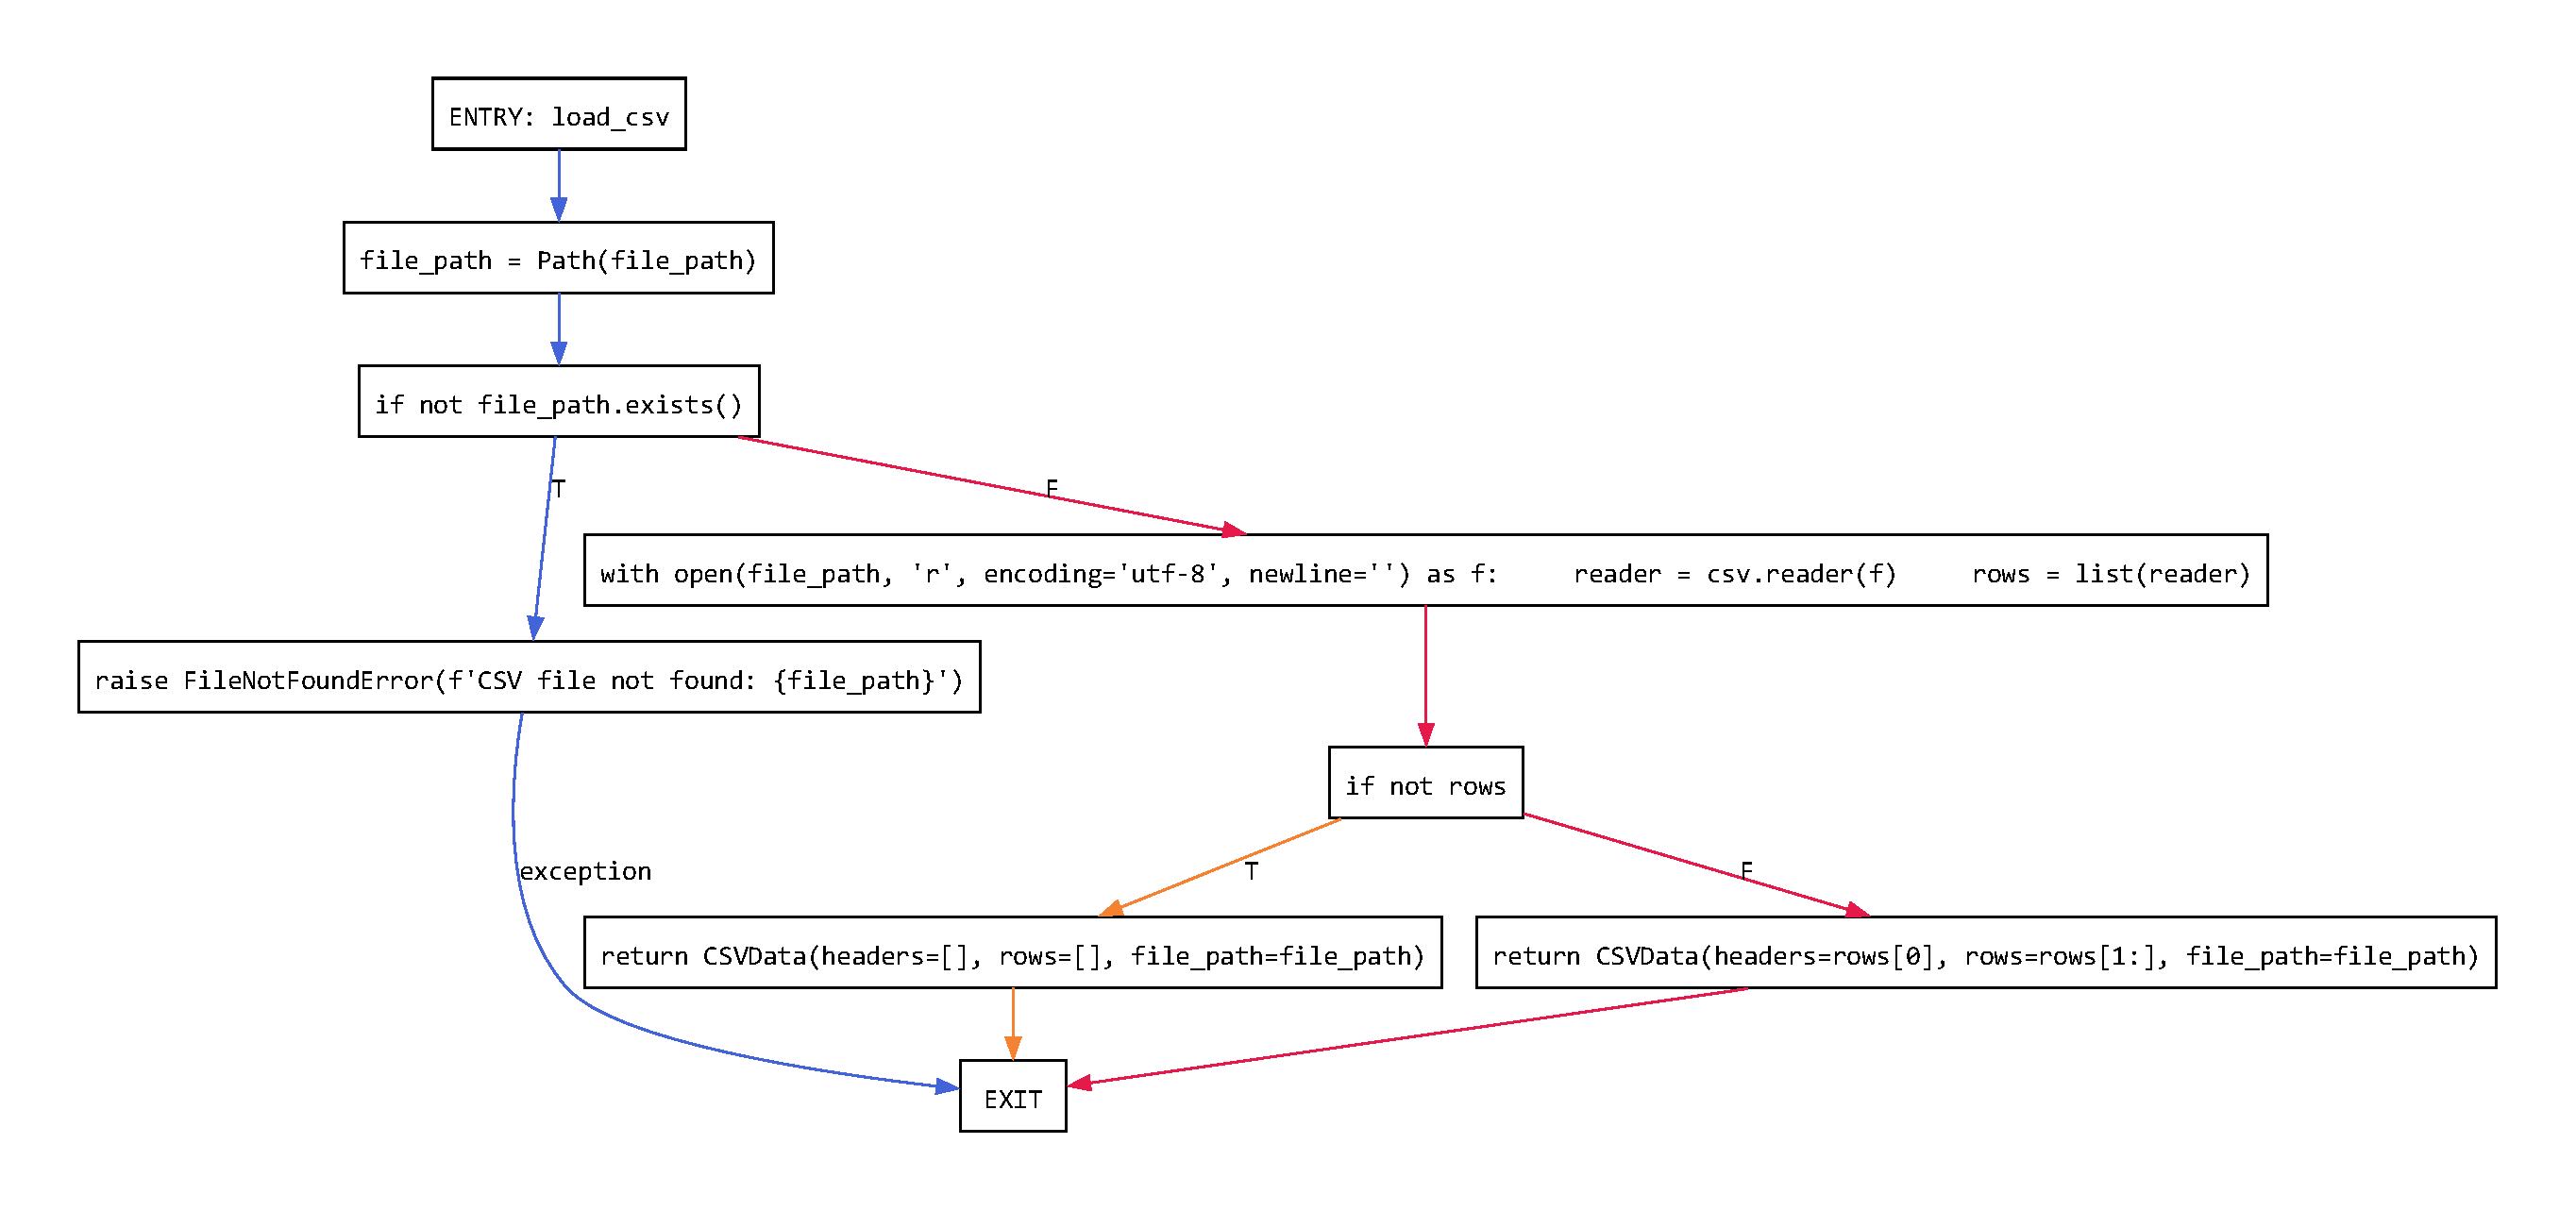
\includegraphics[width=\linewidth]{output-reader-load-csv.pdf}
  \caption{CFG generato per \meth{OutputReader.load\_csv}}
  \label{fig:cfg-loadcsv}
\end{figure}

\begin{table}[H]
  \centering\small
  \caption{Path coperti sul CFG di \cref{fig:cfg-loadcsv}}
  \label{tab:paths}
  \begin{tabularx}{\linewidth}{@{}L{1.5cm} L{2.6cm} Y@{}}
    \toprule
    \thead{Path} & \thead{Test case} & \thead{Comportamento}\\
    \midrule
    P1 & UT-CR2-06 & File non esistente $\rightarrow$ solleva
      \code{FileNotFoundError}.\\
    P2 & UT-CR2-07 & File CSV valido $\rightarrow$ ritorna \cls{CSVData} con
      headers e righe.\\
    P3 & UT-CR2-08 & File CSV vuoto $\rightarrow$ ritorna \cls{CSVData} vuoto.\\
    \bottomrule
  \end{tabularx}
\end{table}

\begin{keypoints}
Tutti i CFG utilizzati nella progettazione white-box sono versionati come
sorgenti Graphviz sotto \pkgpath{test/white\_box\_paths/} e sono rigenerabili in
formato vettoriale con \cmd{python tools/render\_cfg.py}.
\end{keypoints}

\subsubsection{Coverage (pytest-cov, branch coverage)}
\label{sec:coverage}

La coverage \`e stata calcolata con \textbf{pytest-cov}~\cite{pytestcov}
limitatamente alle \textbf{classi di interesse} --- quelle effettivamente
testate in white-box --- misurando in particolare la \textbf{branch coverage}
con soglia obiettivo $\geq 80\%$.

\begin{table}[H]
  \centering\small
  \caption{Branch coverage sulle classi target, per livello di test}
  \label{tab:cov}
  \begin{tabularx}{\linewidth}{@{}L{5.6cm} C{2.6cm} C{2.6cm} Y@{}}
    \toprule
    \thead{Package/Classe} & \thead{Unit} & \thead{Integration} & \thead{CR}\\
    \midrule
    \pkgpath{modules/analyzer/ml\_analyzer.py} &
      98\,\% (43/44) & 100\,\% (44/44) & CR1\\
    \pkgpath{gui/services/pipeline\_service.py} &
      100\,\% (10/10) & 100\,\% (10/10) & CR2\\
    \pkgpath{gui/services/output\_reader.py} &
      93\,\% (13/14) & 93\,\% (13/14) & CR2/CR3\\
    \pkgpath{gui/controller.py} &
      --- & 68\,\% (19/28) & CR2/CR3\\
    \midrule
    \textbf{Totale} & \tagok{97\,\% (66/68)} & \tagok{90\,\% (86/96)} & \\
    \bottomrule
  \end{tabularx}
\end{table}

Lo Unit Testing supera l'obiettivo del Master Test Plan ($\geq 80\%$) su
tutte le classi target. Nell'Integration Testing lo superano tre classi su
quattro: \pkgpath{gui/controller.py} si ferma al 68\,\%. I valori sono
riproducibili con \cmd{pytest -{}-cov} e i report HTML completi generati da
\textbf{coverage.py} sono versionati sotto \pkgpath{docs/coverage/}.

\subsection{Post-Modification System Testing}
\label{sec:st}

Il system testing \`e condotto in modalit\`a \textbf{black-box}, progettando i
casi di test tramite \textbf{Category Partition} secondo il procedimento
descritto in \cref{sec:catpart}. Sono stati definiti tre casi d'uso dedicati
alle nuove funzionalit\`a: UC-CR1 (metriche), UC-CR2 (GUI) e UC-CR3 (dashboard).

\subsubsection{UC-CR1 --- Analisi del calcolo delle metriche}
\label{sec:st-cr1}

\begin{table}[H]
  \centering\small
  \caption{UC-CR1 --- Calcolo delle metriche}
  \label{tab:uc-cr1}
  \begin{tabularx}{\linewidth}{@{}L{3.3cm} Y@{}}
    \toprule
    \thead{Descrizione} & L'utente esegue l'analisi su una directory locale
      contenente repository gi\`a disponibili; il tool calcola le metriche
      Maintainability Index (MI) e Cyclomatic Complexity (CC) per i progetti
      contenuti, salvando i risultati in \pkgpath{io/output/}.\\
    \midrule
    \thead{Attori} & Utente (ricercatore)\\
    \midrule
    \thead{Entry condition} & \file{main\_args.py} disponibile; dipendenze
      installate (inclusa Radon); directory \flag{--repository-path}
      accessibile (per scenari ``success'').\\
    \midrule
    \thead{Exit condition} &
      \emph{Successo}: metriche (MI, CC) calcolate e risultati salvati in
      \pkgpath{io/output/}.\newline
      \emph{Errore}: messaggio d'errore e assenza di output significativo.\\
    \midrule
    \thead{Flusso di eventi principale} &
      1. Invocazione con \flag{--repository-path} e \flag{--metrics}.\newline
      2. Validazione del path.\newline
      3. Scansione dei repository nella directory.\newline
      4. Calcolo MI e CC sui progetti analizzati.\newline
      5. Salvataggio output metriche in \pkgpath{io/output/}.\\
    \bottomrule
  \end{tabularx}
\end{table}

\textbf{Parametro}: path della directory contenente i repository
(\flag{repository\_path}). \quad
\textbf{Oggetti dell'ambiente}: filesystem, contenuto dei progetti.

\begin{table}[H]
  \centering\small
  \caption{UC-CR1 --- Categorie e scelte}
  \label{tab:st-cr1-cat}
  \begin{tabularx}{\linewidth}{@{}L{3.2cm} L{1.2cm} L{5.0cm} Y@{}}
    \toprule
    \thead{Categoria} & \thead{ID} & \thead{Descrizione} &
    \thead{Propriet\`a / Vincoli}\\
    \midrule
    \multirow{2}{=}{Esistenza input directory}
      & ED1 & Directory non esiste & [Error]\\
      & ED2 & Directory esiste     & [property DirOk]\\
    \midrule
    \multirow{2}{=}{Contenuto directory}
      & CD0 & Directory vuota (0 progetti) & [if DirOk] [property Empty]\\
      & CD1 & Directory con 1+ progetti    & [if DirOk] [property MultiProject]\\
    \midrule
    \multirow{4}{=}{Composizione progetti}
      & CP0 & Tutti i progetti senza file Python & [if DirOk and MultiProject]\\
      & CP1 & Tutti i progetti con file Python ma vuoti & [if DirOk and MultiProject]\\
      & CP2 & Tutti i progetti con file Python validi e con codice & [if DirOk and MultiProject]\\
      & CP3 & Mix di progetti validi e non validi & [if DirOk and MultiProject]\\
    \bottomrule
  \end{tabularx}
\end{table}

\begin{table}[H]
  \centering\small
  \caption{UC-CR1 --- Test frame}
  \label{tab:st-cr1-tf}
  \begin{tabularx}{\linewidth}{@{}L{1.3cm} L{3.4cm} Y@{}}
    \toprule
    \thead{ID} & \thead{Combinazioni} & \thead{Oracolo (risultato atteso)}\\
    \midrule
    TF1 & ED1            & Messaggio di errore ``Input folder not found''\\
    TF2 & ED2, CD0       & Nessuna metrica calcolata\\
    TF3 & ED2, CD1, CP0  & Per tutti i progetti MI e CC pari a 0\\
    TF4 & ED2, CD1, CP1  & Per tutti i progetti MI e CC pari a 0\\
    TF5 & ED2, CD1, CP2  & Per tutti i progetti MI e CC sono valori esatti\\
    TF6 & ED2, CD1, CP3  & Per tutti i progetti MI e CC sono valori esatti\\
    \bottomrule
  \end{tabularx}
\end{table}

\begin{longtable}{@{}L{1.2cm} L{3.0cm} L{3.8cm} L{6.5cm}@{}}
  \caption{UC-CR1 --- Test case}\label{tab:st-cr1-tc}\\
  \toprule
  \thead{TC} & \thead{Input (\flag{repository\_path})} &
  \thead{Descrizione ambiente} & \thead{Oracolo}\\
  \midrule
  \endfirsthead
  \toprule
  \thead{TC} & \thead{Input (\flag{repository\_path})} &
  \thead{Descrizione ambiente} & \thead{Oracolo}\\
  \midrule
  \endhead
  \bottomrule
  \endfoot
  TC1 & \file{repo\_does\_not\_exist} & Directory inesistente &
    Messaggio ``Input folder not found''\\
  TC2 & \file{empty\_repo} & Directory vuota & Nessuna metrica calcolata\\
  TC3 & \file{test\_repos/TC3} & Pi\`u progetti senza file Python &
    Per tutti i progetti MI e CC pari a 0\\
  TC4 & \file{test\_repos/TC4} & Pi\`u progetti con file Python vuoti &
    Per tutti i progetti MI e CC pari a 0\\
  TC5 & \file{test\_repos/TC5} & Pi\`u progetti con file Python contenenti
    codice valido &
    Valori esatti calcolati manualmente:\newline
    \code{project1}: CC\_avg $=1{,}67$, MI\_avg $=77{,}5$\newline
    \code{project2}: CC\_avg $=1{,}33$, MI\_avg $=88{,}75$\\
  TC6 & \file{test\_repos/TC6} & Mix: progetti senza file Python, con file
    Python vuoti e con codice valido &
    Valori esatti per ogni progetto:\newline
    \code{project\_empty\_python\_1}: CC\_avg $=0$, MI\_avg $=0$\newline
    \code{project\_empty\_python\_2}: CC\_avg $=0$, MI\_avg $=0$\newline
    \code{project\_no\_python\_1}: CC\_avg $=0$, MI\_avg $=0$\newline
    \code{project\_no\_python\_2}: CC\_avg $=0$, MI\_avg $=0$\newline
    \code{project1}: CC\_avg $=1{,}67$, MI\_avg $=77{,}51$\newline
    \code{project2}: CC\_avg $=1{,}33$, MI\_avg $=88{,}75$\\
\end{longtable}

\subsubsection{UC-CR2 --- Configurazione e avvio analisi tramite GUI}
\label{sec:st-cr2}

\begin{table}[H]
  \centering\small
  \caption{UC-CR2 --- Configurazione ed esecuzione da GUI}
  \label{tab:uc-cr2}
  \begin{tabularx}{\linewidth}{@{}L{3.3cm} Y@{}}
    \toprule
    \thead{Descrizione} & L'utente configura i parametri della pipeline nella
      GUI e avvia l'analisi; al termine il sistema salva i risultati in
      \pkgpath{io/output/} e mostra l'esito (successo/errore).\\
    \midrule
    \thead{Attori} & Utente (ricercatore)\\
    \midrule
    \thead{Entry condition} & GUI aperta; utente nella tab Configuration;
      interfaccia in stato Idle (pulsante Start Analysis abilitato).\\
    \midrule
    \thead{Exit condition} &
      \emph{Successo}: pipeline completata, risultati salvati in
      \pkgpath{io/output/}, dialogo di successo mostrato, interfaccia in stato
      Idle sulla tab Output.\newline
      \emph{Errore}: pipeline fallita o non avviata, dialogo di
      errore/validazione mostrato, interfaccia in stato Idle sulla tab
      Configuration.\\
    \midrule
    \thead{Flusso di eventi principale} &
      1. L'utente imposta i path (IO Path, Repository Path, Project List Path),
         il numero di repo da clonare, seleziona i pipeline step e l'opzione
         Enable Rules 3.\newline
      2. L'utente avvia l'analisi con Start Analysis.\newline
      3. Il sistema valida i parametri, disabilita Start Analysis e avvia la
         pipeline in un thread separato.\newline
      4. Il sistema completa l'analisi, salva i risultati e mostra un dialogo
         di successo.\\
    \bottomrule
  \end{tabularx}
\end{table}

\textbf{Parametri}:

\begin{itemize}[nosep]
  \item \flag{io\_path}, \flag{repos\_path}, \flag{project\_list\_path}
    (String);
  \item \flag{num\_repos} (Integer, 1--1000);
  \item \flag{clone\_enabled}, \flag{verify\_enabled},
    \flag{producer\_enabled}, \flag{consumer\_enabled},
    \flag{metrics\_enabled}, \flag{rules3\_enabled} (Boolean).
\end{itemize}

\textbf{Oggetti dell'ambiente}: stato del filesystem; contenuto e validit\`a del
file CSV dei progetti; stato della cartella contenente i repository.

\begin{longtable}{@{}L{3.4cm} L{1.3cm} L{4.4cm} L{5.4cm}@{}}
  \caption{UC-CR2 --- Categorie e scelte}\label{tab:st-cr2-cat}\\
  \toprule
  \thead{Categoria} & \thead{ID} & \thead{Descrizione} & \thead{Vincoli}\\
  \midrule
  \endfirsthead
  \toprule
  \thead{Categoria} & \thead{ID} & \thead{Descrizione} & \thead{Vincoli}\\
  \midrule
  \endhead
  \bottomrule
  \endfoot
  \multirow{3}{=}{Step selezionati}
    & ST0 & Nessuno step selezionato    & [Single]\\
    & ST1 & Almeno uno step selezionato & [property PARTIAL]\\
    & ST2 & Tutti gli step selezionati  & [property ALL] [Single]\\
  \midrule
  \multirow{2}{=}{Cloning + Verify}
    & CV1 & Cloning e Verify selezionati     & [if PARTIAL] [property CV\_ON]\\
    & CV2 & Cloning e Verify non selezionati & [if PARTIAL] [property CV\_OFF]\\
  \midrule
  \multirow{2}{=}{Esistenza IO directory}
    & IO0 & IO directory non esiste & [Error]\\
    & IO1 & IO directory esiste     & [property IO\_OK]\\
  \midrule
  \multirow{2}{=}{Esistenza directory repo}
    & RP0 & Directory repo non esiste & [Single]\\
    & RP1 & Directory repo esiste     & [property REPO\_OK]\\
  \midrule
  \multirow{2}{=}{Esistenza file CSV}
    & CSV0 & File CSV non esiste & [if CV\_ON and IO\_OK and REPO\_OK] [Error]\\
    & CSV1 & File CSV esiste     & [if CV\_ON and IO\_OK and REPO\_OK] [property CSV\_OK]\\
  \midrule
  \multirow{2}{=}{Stato CSV}
    & CS0 & File CSV vuoto & [if CSV\_OK] [Single] [property CSV\_EMPTY]\\
    & CS1 & File CSV non vuoto, almeno una riga & [if CSV\_OK] [property CSV\_NONEMPTY]\\
  \midrule
  \multirow{2}{=}{Rule 3}
    & RU3\_0 & Regola 3 non selezionata & [property RU3\_OFF] [Single]\\
    & RU3\_1 & Regola 3 selezionata     & [property RU3\_ON] [Single]\\
  \midrule
  \multirow{4}{=}{Valore N-repos}
    & N1 & N-repos $<0$ & [if CSV\_NONEMPTY and CV\_ON] [Error]\\
    & N2 & N-repos $=0$ & [if CSV\_NONEMPTY and CV\_ON] [Single]\\
    & N3 & $0 <$ N-repos $<$ \#righeCSV & [if CSV\_NONEMPTY and CV\_ON] [property N\_OK]\\
    & N4 & N-repos $>$ \#righeCSV & [if CSV\_NONEMPTY and CV\_ON] [Error] [property N\_GT]\\
\end{longtable}

\begin{longtable}{@{}L{1.3cm} L{6.0cm} L{7.6cm}@{}}
  \caption{UC-CR2 --- Test frame}\label{tab:st-cr2-tf}\\
  \toprule
  \thead{ID} & \thead{Combinazioni (categorie/scelte)} &
  \thead{Oracolo (risultato atteso)}\\
  \midrule
  \endfirsthead
  \toprule
  \thead{ID} & \thead{Combinazioni} & \thead{Oracolo}\\
  \midrule
  \endhead
  \bottomrule
  \endfoot
  TF1  & ST0                                    & [Single] Nessuno step\\
  TF2  & ST1, CV1, IO0                          & [Error] IO dir non esiste\\
  TF3  & ST1, CV1, IO1, RP0                     & [Single] Repo dir non esiste e viene creata\\
  TF4  & ST1, CV1, IO1, RP1, CSV0               & [Error] CSV mancante\\
  TF5  & ST1, CV1, IO1, RP1, CSV1, CS0, RU3\_0  & [Single] Regola 3 non eseguita e analisi completata con successo\\
  TF6  & ST1, CV1, IO1, RP1, CSV1, CS0, RU3\_1  & [Single] Regola 3 eseguita e analisi completata con successo\\
  TF7  & ST1, CV1, IO1, RP1, CSV1, CS1, N1      & [Error] N-repos $<0$\\
  TF8  & ST1, CV1, IO1, RP1, CSV1, CS1, N2      & [Single] N-repos $=0$ e analisi completata con successo\\
  TF9  & ST1, CV1, IO1, RP1, CSV1, CS1, N3      & Analisi completata con successo\\
  TF10 & ST1, CV1, IO1, RP1, CSV1, CS1, N4      & [Error] N-repos $>$ \#righeCSV\\
  TF11 & ST1, CV2, IO1, RP1                     & Analisi completata con successo (solo step Producer)\\
  TF12 & ST2, CV1, IO1, RP1, CSV1, CS1, N3      & [Single] Tutti gli step eseguiti e analisi completata con successo\\
\end{longtable}

I dodici test frame sono stati istanziati in altrettanti test case eseguibili,
implementati in \file{test/system\_testing/gui\_test/gui\_test.py}. Ogni test
case pilota la GUI reale impostando i parametri, avviando la pipeline e
verificando lo stato dell'interfaccia e i dialoghi mostrati.

\begin{table}[H]
  \centering\small
  \caption{UC-CR2 --- Esempio di test case (TF11 e TF12)}
  \label{tab:st-cr2-tc}
  \begin{tabularx}{\linewidth}{@{}L{1.2cm} L{4.3cm} L{4.0cm} Y@{}}
    \toprule
    \thead{TC} & \thead{Input} & \thead{Descrizione ambiente} &
    \thead{Oracolo}\\
    \midrule
    TC11 & Solo \emph{Producer} selezionato.\newline
      Directory IO: \file{temp\_io\_structure}.\newline
      Directory repo: \file{repos}. &
      Directory IO esiste. Directory repo esiste. &
      Solo lo step \emph{Producer} abilitato.\newline
      Titolo: `Success'; messaggio: `Pipeline completed successfully!'.\\
    TC12 & Tutti gli step selezionati.\newline
      Directory IO: \file{temp\_io\_structure}.\newline
      Directory repo: \file{repos}.\newline
      File CSV: \file{projects\_TF12.csv}. Numero repos: 3. &
      Directory IO e repo esistono. Il CSV contiene
      \code{owner1/project1} \ldots \code{owner5/project5}. &
      Tutti gli step eseguiti.\newline
      Titolo: `Success'; messaggio: `Pipeline completed successfully!'.\\
    \bottomrule
  \end{tabularx}
\end{table}

\begin{keypoints}
\textbf{Nota sull'implementazione.} Al fine di semplificare la definizione e
l'esecuzione dei test case sono state sviluppate \textbf{6 funzioni di
utilit\`a}. Tali funzioni sono state a loro volta testate, ma i relativi
dettagli sono omessi dal presente documento e non sono conteggiati nei totali di
\cref{tab:ripartizione}.
\end{keypoints}

\subsubsection{UC-CR3 --- Consultazione delle analisi tramite dashboard}
\label{sec:st-cr3}

\begin{table}[H]
  \centering\small
  \caption{UC-CR3 --- Consultazione della dashboard}
  \label{tab:uc-cr3}
  \begin{tabularx}{\linewidth}{@{}L{3.3cm} Y@{}}
    \toprule
    \thead{Descrizione} & L'utente accede alla tab Dashboard della GUI,
      seleziona una delle analisi disponibili e ne visualizza i risultati in
      forma grafica e aggregata (overview, metriche e top librerie).\\
    \midrule
    \thead{Attori} & Utente (ricercatore)\\
    \midrule
    \thead{Entry condition} & GUI aperta; utente nella tab Dashboard;
      interfaccia in stato Idle.\\
    \midrule
    \thead{Exit condition} &
      \emph{Successo}: analisi selezionata visualizzata correttamente;
      interfaccia in stato Idle sulla tab Dashboard.\newline
      \emph{Errore}: errore imprevisto o visualizzazione fallita; interfaccia in
      stato Idle sulla tab Dashboard con messaggio di errore mostrato.\\
    \midrule
    \thead{Flusso di eventi principale} &
      1. Il sistema mostra l'elenco delle analisi disponibili e attende una
         selezione.\newline
      2. L'utente seleziona un'analisi (ad es.\ \code{Analysis\_1}).\newline
      3. Il sistema visualizza Analysis Overview (conteggi e percentuali
         Producer/Consumer/Producer\,\&\,Consumer), Code Quality Metrics
         (CC e MI medi) e Top 10 ML Libraries Detected.\\
    \bottomrule
  \end{tabularx}
\end{table}

\textbf{Parametri}: \pkgpath{io/output/producer} e \pkgpath{io/output/consumer}
(percorsi contenenti i risultati delle analisi per producer e consumer);
\pkgpath{io/output/metrics} (percorso contenente i risultati per le metriche CC
e MI). \quad \textbf{Oggetti dell'ambiente}: stato del filesystem.

\begin{table}[H]
  \centering\small
  \caption{UC-CR3 --- Categorie e scelte}
  \label{tab:st-cr3-cat}
  \begin{tabularx}{\linewidth}{@{}L{3.8cm} L{1.4cm} L{5.2cm} Y@{}}
    \toprule
    \thead{Categoria} & \thead{ID} & \thead{Descrizione} &
    \thead{Propriet\`a}\\
    \midrule
    \multirow{2}{=}{Directory producer e consumer}
      & DPC0 & Directory vuote (0 risultati per progetti producer e consumer)
             & [property DirProConEmp]\\
      & DPC1 & Directory con 1+ risultati per progetti producer e consumer
             & [property DirProMulPro]\\
    \midrule
    \multirow{2}{=}{Directory metrics}
      & DM0 & Directory vuota (0 progetti analizzati) & [property DirMetEmp]\\
      & DM1 & Directory con 1+ risultati per progetti analizzati
            & [property DirMetMulPro]\\
    \bottomrule
  \end{tabularx}
\end{table}

\begin{table}[H]
  \centering\small
  \caption{UC-CR3 --- Test frame}
  \label{tab:st-cr3-tf}
  \begin{tabularx}{\linewidth}{@{}L{1.3cm} L{2.6cm} Y@{}}
    \toprule
    \thead{ID} & \thead{Combinazioni} & \thead{Oracolo (risultato atteso)}\\
    \midrule
    TF1 & DPC0, DM0 & Non compare nessuna Analysis\\
    TF2 & DPC0, DM1 & Compare Analysis; selezionandola mostra la media delle
      metriche dei progetti in input, mentre i restanti valori sono pari a 0\\
    TF3 & DPC1, DM0 & Compare Analysis; selezionandola mostra il numero di
      consumer e producer corrispondenti e le keyword pi\`u usate, mentre i
      restanti valori sono pari a 0\\
    TF4 & DPC1, DM1 & Compare Analysis; selezionandola mostra numero di
      consumer e producer, le keyword pi\`u usate e la media delle metriche\\
    \bottomrule
  \end{tabularx}
\end{table}

I quattro test frame sono stati istanziati in altrettanti test case,
implementati in \file{test/system\_testing/dashboard\_test/dashboard\_test.py}.
Ogni test case popola le directory di output con CSV controllati, apre la
dashboard e verifica le etichette del Classification Summary, i valori di Code
Metrics e il contenuto della tabella ML Keywords Usage.

\subsection{Regression Testing}
\label{sec:regression}

Il regression testing \`e stato condotto tramite la riesecuzione completa della
suite di test preesistente, in particolare i test di sistema eseguiti nella fase
pre-modifica (\cref{sec:premod}): \textbf{16 test case} definiti sui due casi
d'uso principali (UC-1 Analysis: 12 test case; UC-2 Cloning: 4 test case) e
completati senza fallimenti prima delle modifiche.

\begin{table}[H]
  \centering\small
  \caption{Riepilogo della nuova esecuzione della suite di regressione}
  \label{tab:regression}
  \begin{tabularx}{0.75\linewidth}{@{}Y C{2.4cm} C{2.4cm}@{}}
    \toprule
    \thead{Totale} & \thead{Superati} & \thead{Falliti}\\
    \midrule
    16 & \tagok{16} & \tagok{0}\\
    \bottomrule
  \end{tabularx}
\end{table}

L'esito conferma sul campo il vincolo progettuale enunciato in
\cref{sec:ia-cr23}: le funzionalit\`a preesistenti si comportano esattamente
come prima delle modifiche.

\subsection{Riepilogo dei risultati}
\label{sec:riepilogo-test}

Al termine dell'esecuzione dei vari test, tutti gli \textbf{84 casi di test}
previsti sono stati eseguiti con successo, senza riscontrare alcun fallimento.

\begin{table}[H]
  \centering\small
  \caption{Risultati complessivi}
  \label{tab:risultati}
  \begin{tabularx}{\linewidth}{@{}Y C{2.6cm} C{2.4cm} C{3.4cm}@{}}
    \toprule
    \thead{Test eseguiti} & \thead{Superati} & \thead{Fallimenti} &
    \thead{Incident / anomalie}\\
    \midrule
    84 & \tagok{84} & \tagok{0} & \tagok{Nessuna}\\
    \bottomrule
  \end{tabularx}
\end{table}

\begin{table}[H]
  \centering\small
  \caption{Ripartizione dei test eseguiti}
  \label{tab:ripartizione}
  \begin{tabularx}{\linewidth}{@{}L{4.0cm} L{4.2cm} C{2.8cm} Y@{}}
    \toprule
    \thead{Fase} & \thead{Tipo} & \thead{Riferimento} & \thead{Numero}\\
    \midrule
    \multirow{9}{=}{Test eseguiti post-modification}
      & \multirow{3}{=}{Unit Test}        & CR1 & 8\\
      &                                   & CR2 & 8\\
      &                                   & CR3 & 2\\
    \cmidrule(l){2-4}
      & \multirow{3}{=}{Integration Test} & CR1 & 8\\
      &                                   & CR2 & 13\\
      &                                   & CR3 & 7\\
    \cmidrule(l){2-4}
      & \multirow{3}{=}{System Test (CR1, CR2, CR3)} & CR1 & 6\\
      &                                   & CR2 & 12\\
      &                                   & CR3 & 4\\
    \midrule
    \multirow{2}{=}{Regression Testing}
      & \multirow{2}{=}{System Test Pre-Modification} & UC-1 Analysis & 12\\
      &                                   & UC-2 Cloning & 4\\
    \midrule
    \multicolumn{3}{@{}l}{\textbf{Totale}} & \textbf{84}\\
    \bottomrule
  \end{tabularx}
\end{table}

\begin{keypoints}
\textbf{Corrispondenza con la suite automatizzata.} Eseguendo
\cmd{python -m pytest} l'intera suite raccoglie \textbf{90} test: gli 84 casi
di test documentati qui pi\`u le \textbf{6} funzioni di utilit\`a del
\file{gui\_test} citate in \cref{sec:st-cr2}, che non costituiscono test case
del piano ma sono comunque verificate.
\end{keypoints}

% ===========================================================================
\section{Conclusioni}
\label{sec:conclusioni}

\subsection{Sintesi dei risultati}
\label{sec:sintesi}

Il lavoro ha portato \baselineName{} a \projectName{} attraverso tre Change
Request, tutte rilasciate e verificate. I risultati principali sono riassunti in
\cref{tab:risultati-chiave}, che rimanda ai dati di dettaglio riportati nelle
sezioni precedenti anzich\'e ripeterli.

\begin{table}[H]
  \centering\small
  \caption{Risultati chiave dell'evoluzione \projectName{}}
  \label{tab:risultati-chiave}
  \begin{tabularx}{\linewidth}{@{}L{4.4cm} Y L{2.4cm}@{}}
    \toprule
    \thead{Risultato} & \thead{Descrizione} & \thead{Riferimento}\\
    \midrule
    Integrazione strutturata delle metriche di qualit\`a (CR1) &
      Il core \`e stato esteso con il calcolo automatico di Cyclomatic
      Complexity e Maintainability Index tramite Radon~\cite{radon}, con
      aggregazione a livello di progetto. &
      \cref{sec:cr1}\\
    Introduzione di un layer di configurazione (CR2) &
      La GUI sviluppata in Tkinter consente di configurare ed eseguire l'analisi
      senza ricorrere alla CLI e senza modificare manualmente i parametri
      all'interno del codice. &
      \cref{sec:cr2}\\
    Dashboard grafica integrata (CR3) &
      I risultati sono presentati tramite grafici dinamici (matplotlib) che
      rendono immediata l'interpretazione dei risultati. &
      \cref{sec:cr3}\\
    Impatto stimato e poi misurato &
      L'Impact Analysis della CR1 ha ottenuto recall pari a 1 con precision
      $0{,}77$; per CR2 e CR3 l'impatto sul core \`e nullo per costruzione. &
      \cref{tab:ia-riepilogo}\\
    Elevata copertura di test &
      Le componenti modificate raggiungono il 97\,\% di branch coverage nello
      Unit Testing e il 90\,\% nell'Integration Testing. &
      \cref{tab:cov}\\
    Baseline verificata e stabile &
      Dai due casi d'uso principali \`e stata derivata una suite di 16 system
      test, rieseguita dopo le modifiche senza alcun fallimento. &
      \cref{tab:premod-esito}, \cref{tab:regression}\\
    \bottomrule
  \end{tabularx}
\end{table}

Complessivamente sono stati eseguiti \textbf{84 casi di test} documentati, tutti
superati e senza incident (\cref{tab:risultati}).

\subsection{Valutazione del processo}
\label{sec:valutazione}

Al di l\`a delle funzionalit\`a aggiunte, il progetto ha consolidato un processo
di \textbf{evoluzione controllata} basato su change management, impact analysis e
testing sistematico. Tre osservazioni meritano di essere messe in evidenza.

\paragraph{I falsi positivi come misura dell'estensibilit\`a.}
Il risultato metodologicamente pi\`u interessante riguarda l'Impact Analysis
della CR1. I tre falsi positivi (\meth{MLAnalysisFacade.run\_analysis},
\meth{AnalyzerFactory.create\_builder}, \meth{AnalyzerBuilder.build}) non sono
il sintomo di una stima imprecisa: sono la conferma empirica che i design
pattern gi\`a presenti nella baseline --- in particolare il Factory-Registry ---
erano sufficientemente estensibili da assorbire un nuovo ruolo di analisi senza
alcuna modifica. Una previsione ragionevole ha indicato quei metodi come
candidati; il codice ha dimostrato che non serviva toccarli.

\paragraph{Il valore di un'analisi conservativa.}
La scelta di espandere il call graph sia in fan-in sia in fan-out ha prodotto una
sovra-approssimazione voluta: precision $0{,}77$ a fronte di recall pari a 1
(\cref{eq:precision,eq:recall}). In manutenzione \`e il compromesso desiderabile,
perch\'e i due errori non hanno lo stesso costo --- un falso positivo costa una
verifica in pi\`u, un falso negativo costa un difetto non individuato.

\paragraph{Un vincolo progettuale verificato, non solo dichiarato.}
CR2 e CR3 sono state progettate come strati che invocano il core senza
modificarlo, il che rende l'impatto sui componenti preesistenti nullo \emph{per
costruzione} (\cref{sec:ia-cr23}). Il punto \`e che tale vincolo non \`e rimasto
un'affermazione di progetto: la suite di 16 test di sistema, definita
\emph{prima} di qualunque modifica proprio a questo scopo, lo ha confermato
sperimentalmente al termine del lavoro.

\subsection{Limiti e sviluppi futuri}
\label{sec:futuri}

Il principale limite riguarda la copertura di \pkgpath{gui/controller.py}, che
si ferma al 68\,\% di branch coverage in integrazione e resta quindi
\textbf{sotto l'obiettivo di $\geq 80\%$} fissato dal Master Test Plan
(\cref{sec:mtp-coverage}); le altre tre classi target superano ampiamente la
soglia. Il completamento della copertura sui rami di gestione degli errori del
Controller \`e la prima attivit\`a di verifica da pianificare.

Sul piano funzionale si prevede di:

\begin{itemize}[nosep]
  \item estendere il numero di tipologie di classificazione ML (oltre
    Producer/Consumer);
  \item integrare nuove metriche di qualit\`a (ad es.\ coupling, cohesion);
  \item arricchire la GUI con nuovi grafici e filtri interattivi.
\end{itemize}

% --- Bibliografia ----------------------------------------------------------
\clearpage
\printbibliography[heading=bibnumbered,title={Riferimenti bibliografici}]

\end{document}
